% !TEX root=../../mt-motion-analysis.tex
\chapter{Results and Discussion} \label{ch:results}
\section{Body part localization}
The pose estimation was reliable as long as body parts were not occluded. Figure \ref{fig:occluded} shows a sequence of frames from which it is clear that all body parts except the right foot are found accurately. This figure also suggests this video was not recorded from straight ahead. This is a problem as the plane with the the coordinates will be slightly rotated, resulting in distorted body part positions.

{\addtolength{\textfloatsep}{-0.2in}
\begin{figure}[h]
  \centering
  \begin{subfigure}[t]{0.22\textwidth}
    \centering
    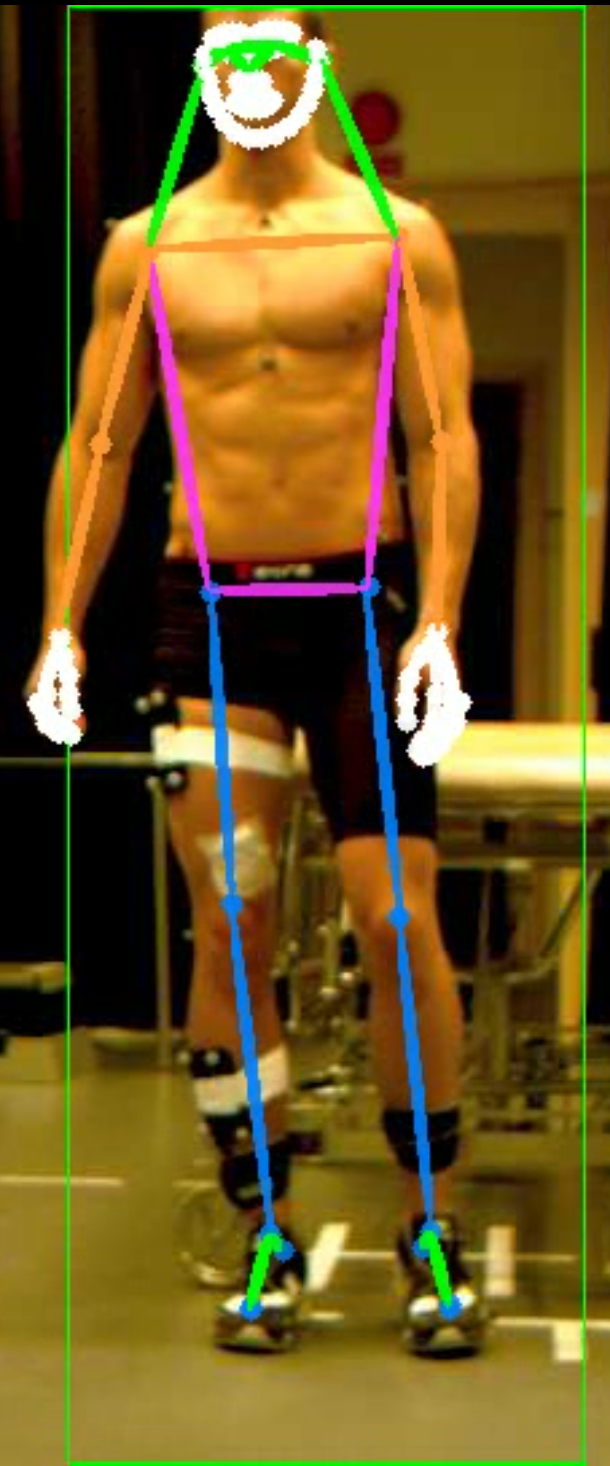
\includegraphics[height=1.3\textwidth]{files/figs/res/hpe/36-1.png}
    \caption{}
  \end{subfigure}
  ~
  \begin{subfigure}[t]{0.22\textwidth}
    \centering
    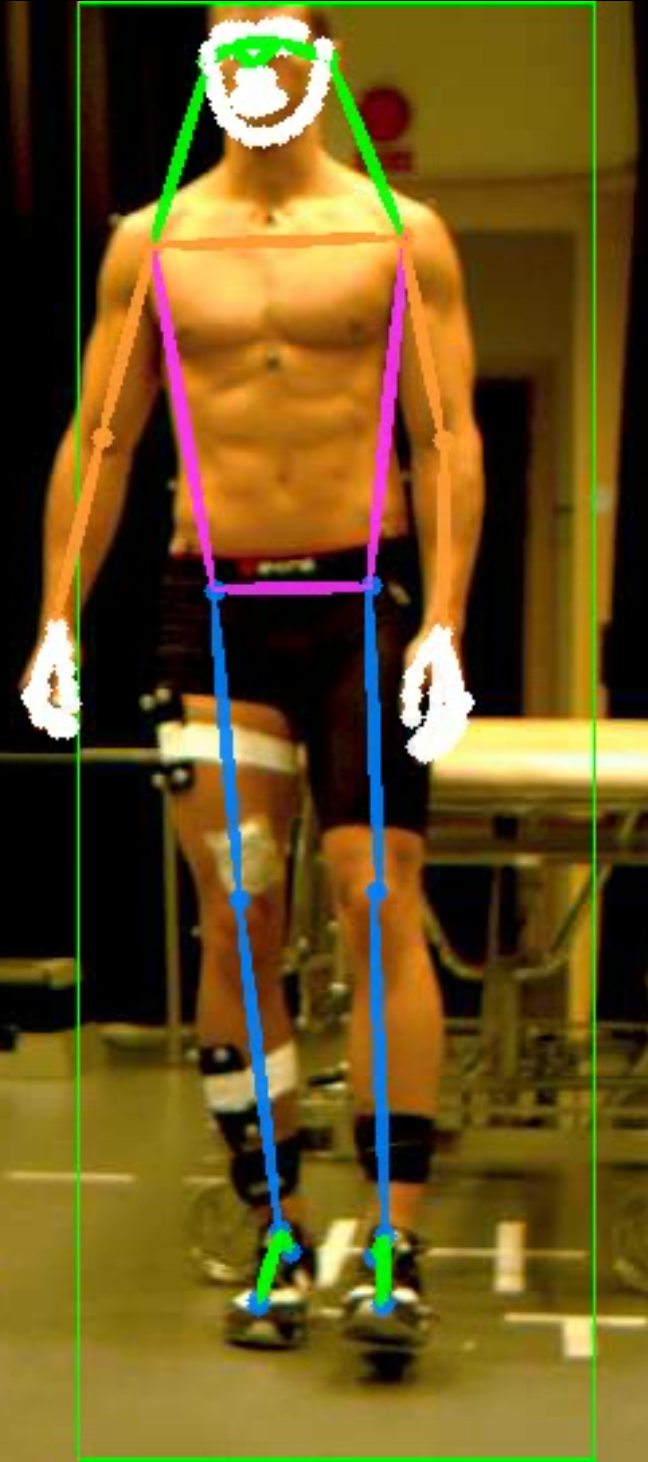
\includegraphics[height=1.3\textwidth]{files/figs/res/hpe/36-2.png}
    \caption{}
  \end{subfigure}
  ~
  \begin{subfigure}[t]{0.22\textwidth}
    \centering
    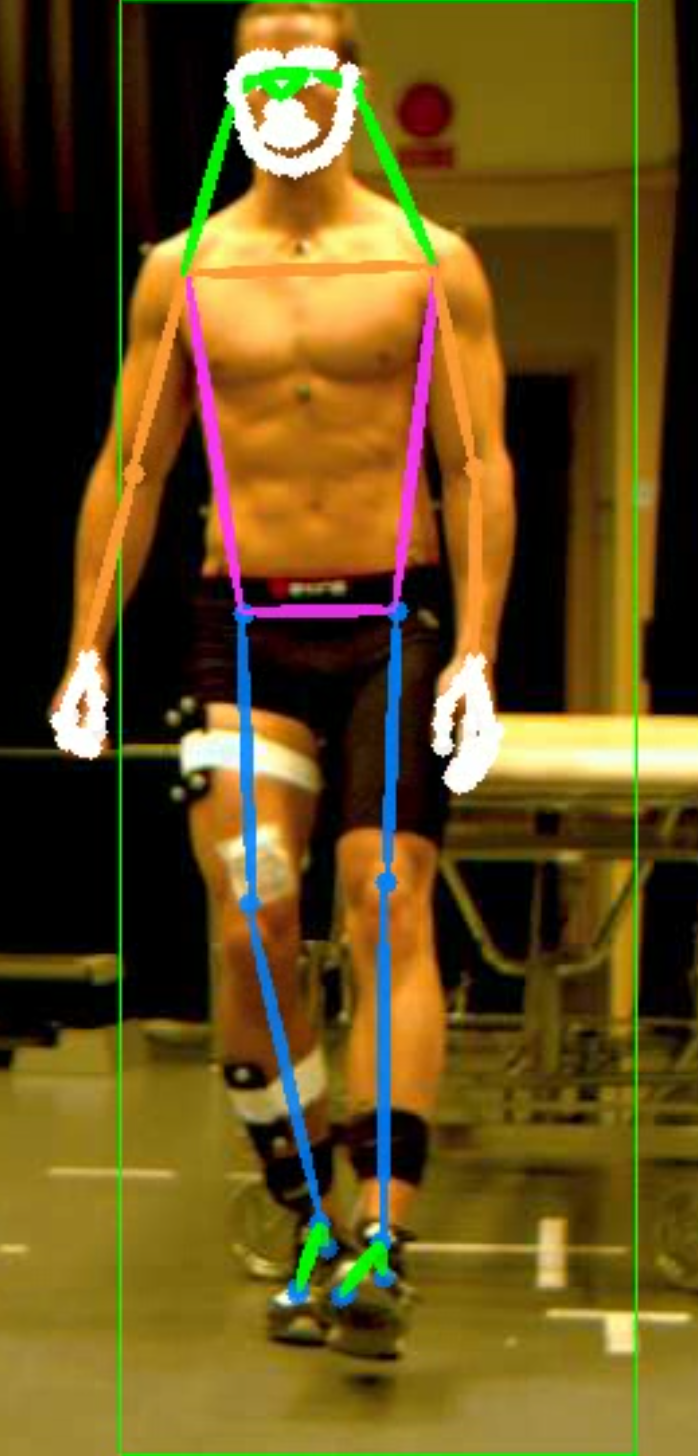
\includegraphics[height=1.3\textwidth]{files/figs/res/hpe/36-3.png}
    \caption{}
  \end{subfigure}
  ~
  \begin{subfigure}[t]{0.22\textwidth}
    \centering
    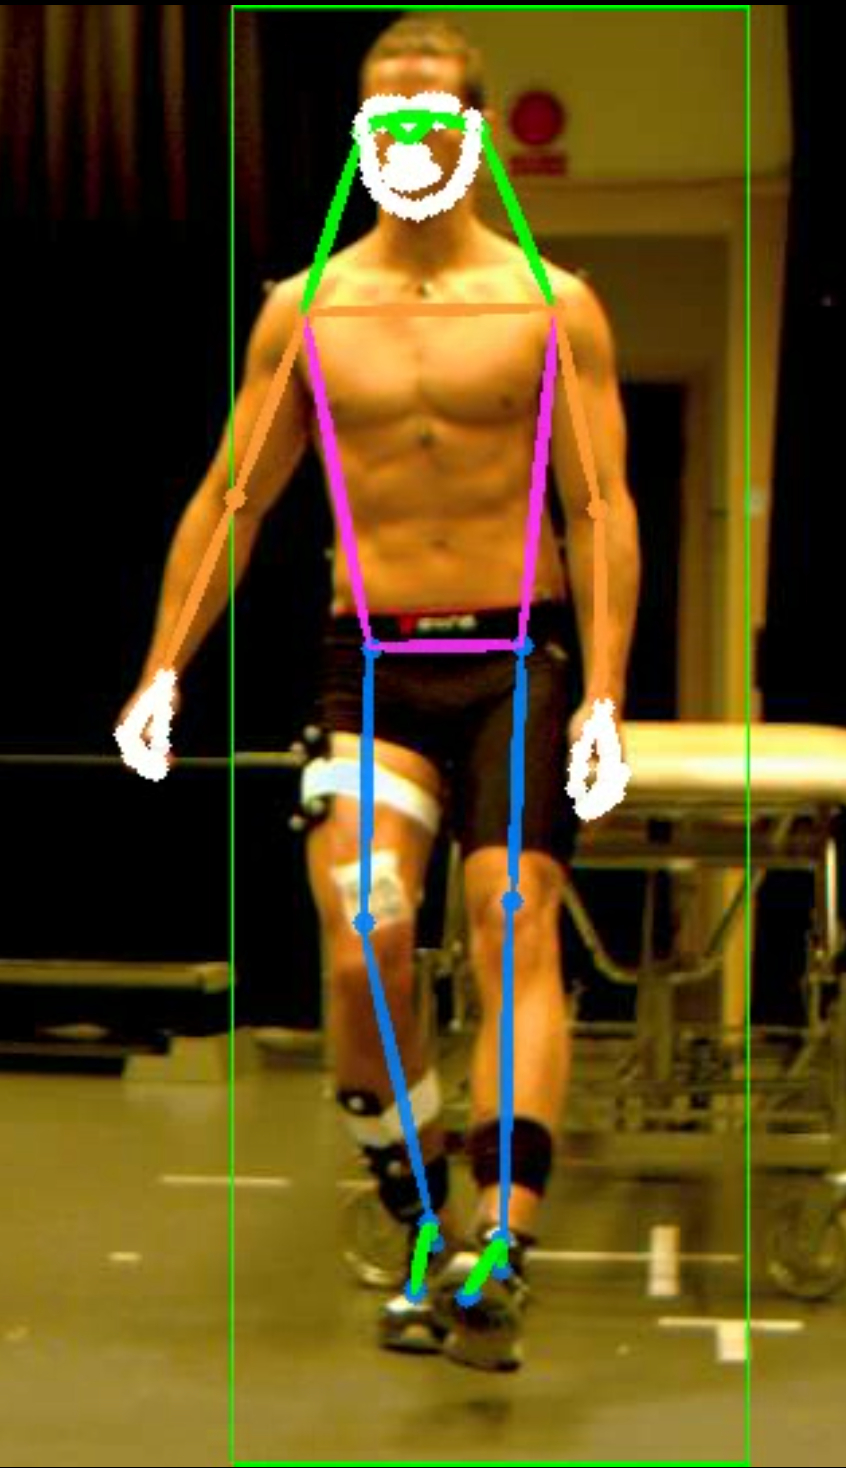
\includegraphics[height=1.3\textwidth]{files/figs/res/hpe/36-4.png}
    \caption{}
  \end{subfigure}

  \begin{subfigure}[t]{0.22\textwidth}
    \centering
    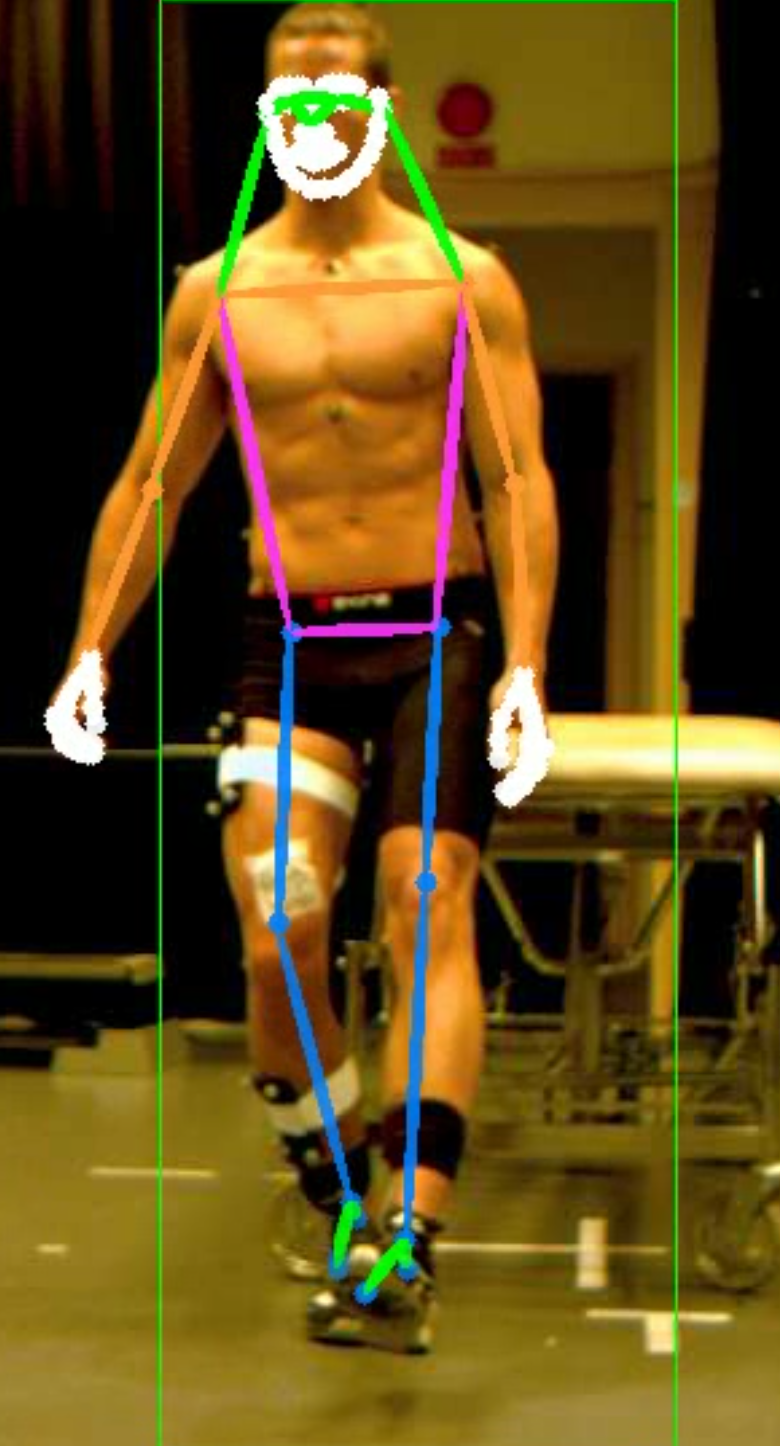
\includegraphics[height=1.3\textwidth]{files/figs/res/hpe/36-5.png}
    \caption{}
  \end{subfigure}
  ~
  \begin{subfigure}[t]{0.22\textwidth}
    \centering
    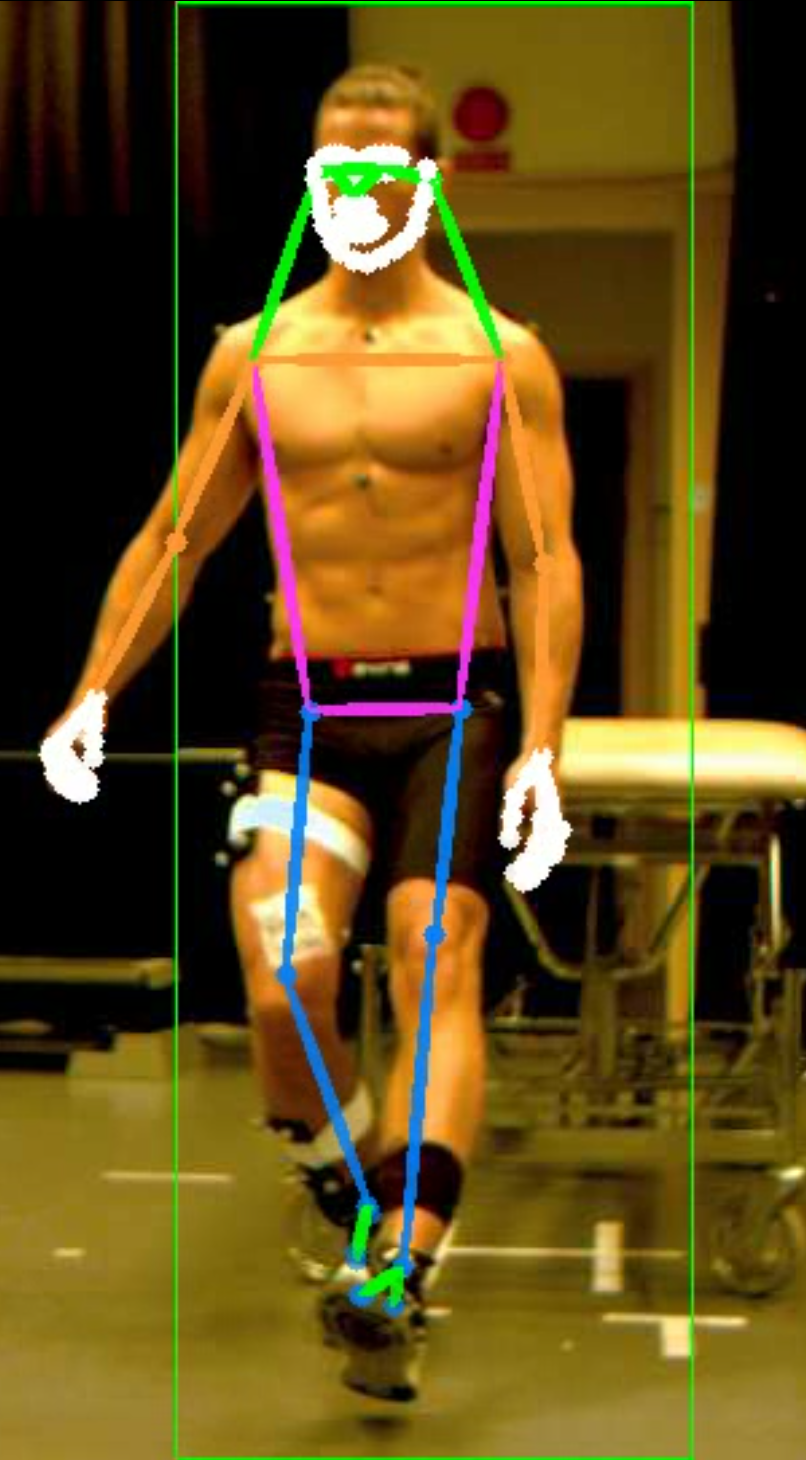
\includegraphics[height=1.3\textwidth]{files/figs/res/hpe/36-6.png}
    \caption{}
  \end{subfigure}
  ~
  \begin{subfigure}[t]{0.22\textwidth}
    \centering
    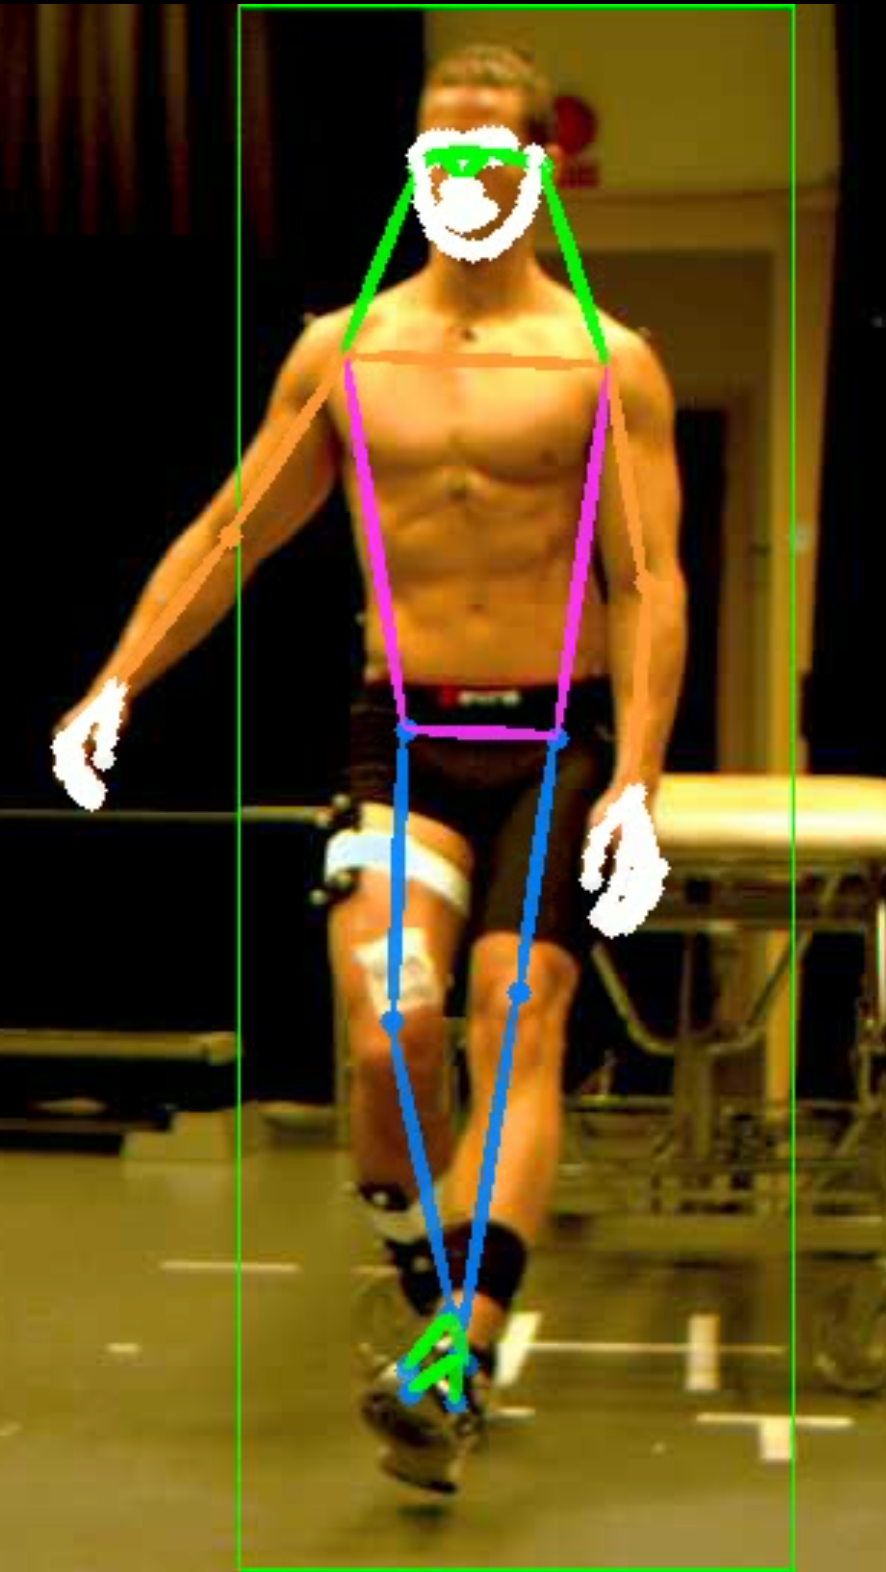
\includegraphics[height=1.3\textwidth]{files/figs/res/hpe/36-7.png}
    \caption{}
  \end{subfigure}
  ~
  \begin{subfigure}[t]{0.22\textwidth}
    \centering
    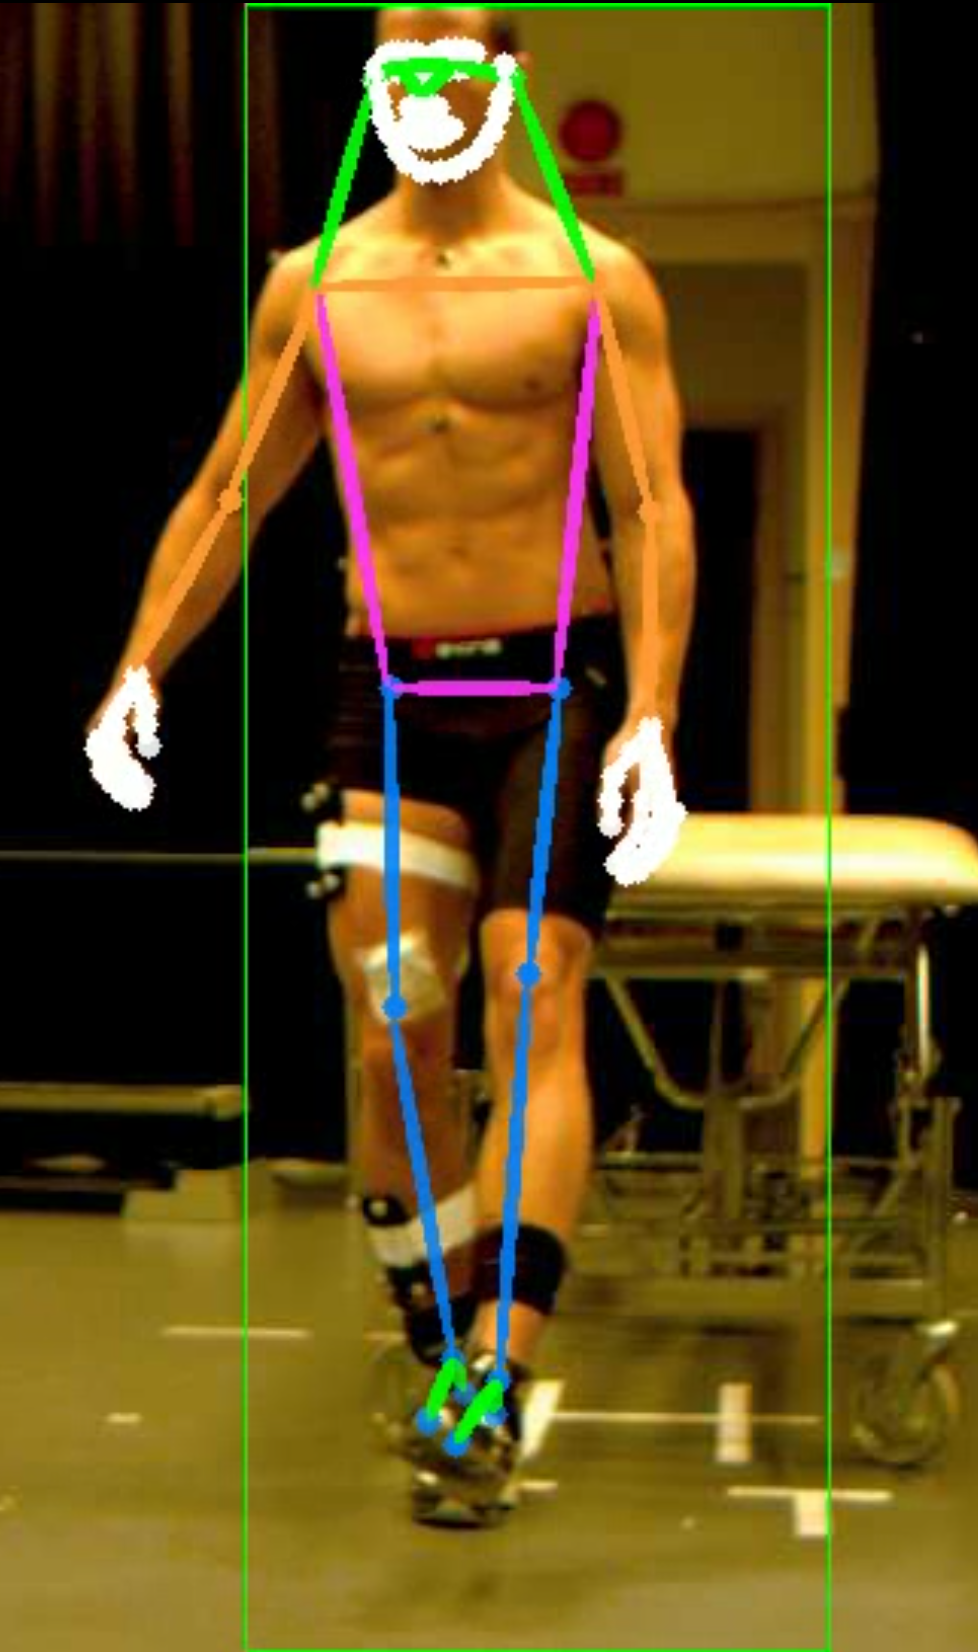
\includegraphics[height=1.3\textwidth]{files/figs/res/hpe/36-8.png}
    \caption{}
  \end{subfigure}

  \caption{Frames from video where the right foot is occluded (c)-(h).}
  \label{fig:occluded}
\end{figure}
}
% + ta fram lite resultat fr[n 3d-data???
% om jag f[r tag p[ mer data att validera mot? annars hur?

\FloatBarrier
\section{Classification}
The figures and results presented in this section are generated by models and ensembles trained according to the cross validation strategy described in Section \ref{sec:met-training} and evaluated on the test set. This results in 10 sets of models trained on slightly different data.

\subsection{Baseline results}
The repetition accuracy and F1 scores for the baseline methods presented in Section~\ref{sec:met-baseline} are shown in Table~\ref{tab:baseline-results}.

\begin{table}[h]
  \centering
  \caption{Baseline results for the different POEs for the classification of the individual repetitions. The results are the mean from the 10 folds $\pm$ the corresponding standard deviations. The F1 score is macro averaged.}
  \label{tab:baseline-results}
  \footnotesize
  \begin{tabu}[c]{|c||c|c||c|c||c|c||c|c|}
    \hline
     \multirow{2}{*}{}& \multicolumn{2}{c||}{\textbf{Trunk}} & \multicolumn{2}{c||}{\textbf{Pelvis}} & \multicolumn{2}{c||}{\textbf{Femoral Valgus}} & \multicolumn{2}{c|}{\textbf{\gls{kmfp}}} \\ \cline{2-9}
    & SVM & LDA & SVM & LDA & SVM & LDA & SVM & LDA \\ \hline %\hline
    Acc(\%) & {\footnotesize 35.3$\pm$5.2&45.2$\pm$5.4&52.3$\pm$4.3&46.2$\pm$3.9&38.6$\pm$3.6 &42.1$\pm$3.5&78.7$\pm$5.8&53.7$\pm$6.8}\\ \hline
    F1(\%) & {\footnotesize 17.3$\pm$1.9&41.5$\pm$5.5&35.5$\pm$3.1&37.9$\pm$3.0&29.6$\pm$2.6&40.6$\pm$3.9&36.7$\pm$2.4&47.1$\pm$9.2}\\ \hline
  \end{tabu}

\end{table}

\subsection{Trunk}
Figure \ref{fig:trunk-cnf-reps}} shows the confusion matrix summarizing the classifications of the individual repetitions made by the ensemble presented in Table \ref{tab:ensemble-models} and Appendix \ref{app:models}.
Each entry in the matrix is the mean along with the standard deviation for models from the 10 folds. Figures \ref{fig:trunk-cnf-comb} and \ref{fig:trunk-cnf-comb-th} shows the corresponding matrices for the combined scores, with and without the threshold suggested in Section~\ref{sec:met-combined}. Figure \ref{fig:trunk-cnf-ignored} shows how the samples ignored due to the threshold were classified.
These results are also summarized as accuracy, F1 scores, precision, and recall in Table \ref{tab:trunk-results}. This table also shows the model performance for the data with different label certainty, specified by the physiotherapist labeling the data. Histograms for these metrics are shown in Figure \ref{fig:trunk-hist-results} along with the corresponding metrics for the individual models in the ensemble (high precision models are not shown as they only predict one label).

\begin{table}[h]
  \centering
  \caption{Results of the ensemble for the trunk POE. Rep., Comb., and Thresh. represents the results for the repetitions, combinations, and combinations with thresholds, respectively. The Certainties columns show the results making up the Comb. column, but for the certainty levels of the expert labeling the data. These ranges from certain (0) to uncertain (2), the variable $n$ shows how many datapoints each category contains. All results are the mean from the 10 folds $\pm$ the corresponding standard deviations. F1, recall, and precision are macro averaged.}
  \label{tab:trunk-results}
  \small
  \begin{tabu}[c]{|c|c|c|c||c|c|c|}
    \hline
    & \multirow{2}{*}{\textbf{Rep.}} & \multirow{2}{*}{\textbf{Comb.}} & \multirow{2}{*}{\textbf{Thresh.}} & \multicolumn{3}{c|}{\textbf{Certainties}}\\ \cline{5-7}
    & & & &0($n$=15)&1($n$=6)&2($n$=1)\\ \hline
    Accuracy (\%)   &73.7$\pm$4.5&75.0$\pm$7.9&\textbf{80.0$\pm$7.8}&
                    81.3$\pm$7.1&56.7$\pm$15.2&textbf{90.0$\pm$30.0}\\ \hline
    F1 score (\%)   &73.1$\pm$3.4&75.0$\pm$5.8&\textbf{79.9$\pm$8.9}&
                    80.4$\pm$7.1&25.8$\pm$6.3&textbf{90.0$\pm$30.0}\\ \hline
    Recall (\%)     &73.3$\pm$3.7&76.7$\pm$3.8&\textbf{81.6$\pm$7.2}&
                    \textbf{81.1$\pm$5.0}&28.0$\pm$11.0&30.0$\pm$10.0\\ \hline
    Precision (\%)  &76.7$\pm$4.1&78.7$\pm$5.2&\textbf{83.0$\pm$6.8}&
                    \textbf{84.9$\pm$5.9}&28.9$\pm$6.8&30.0$\pm$10.0\\ \hline

  \end{tabu}
\end{table}

\begin{figure}[h]
  \centering
  \begin{subfigure}[t]{0.48\textwidth}
      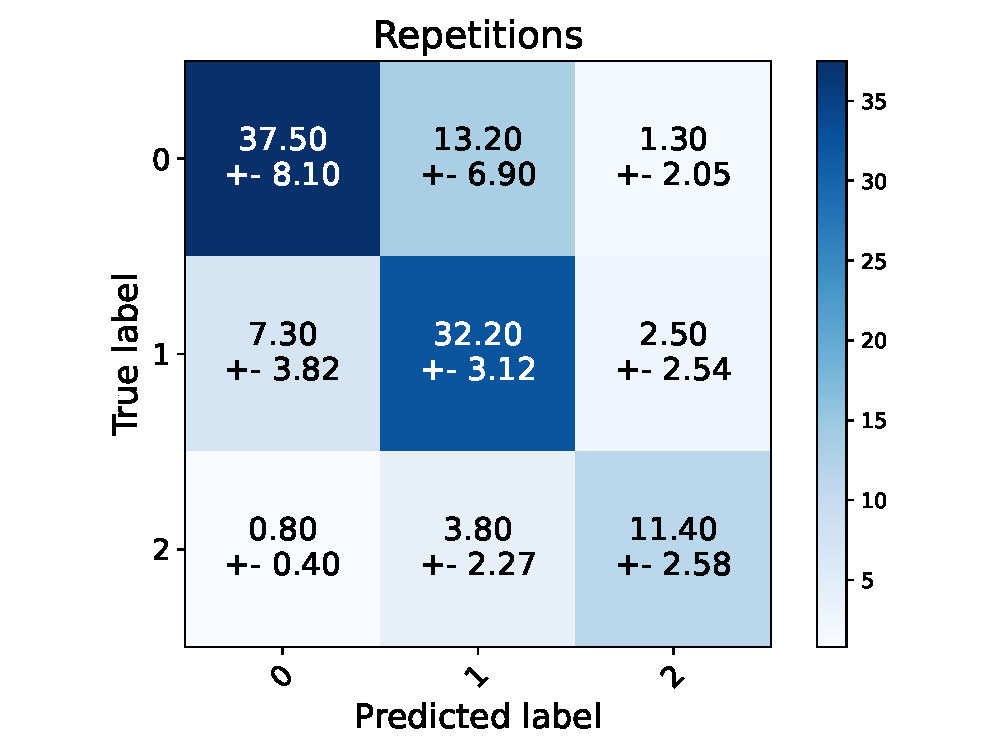
\includegraphics[width=\textwidth]{files/figs/res/trunk/cnf-reps.eps}
      \caption{}
      \label{fig:trunk-cnf-reps}
  \end{subfigure}
  ~
  \begin{subfigure}[t]{0.48\textwidth}
      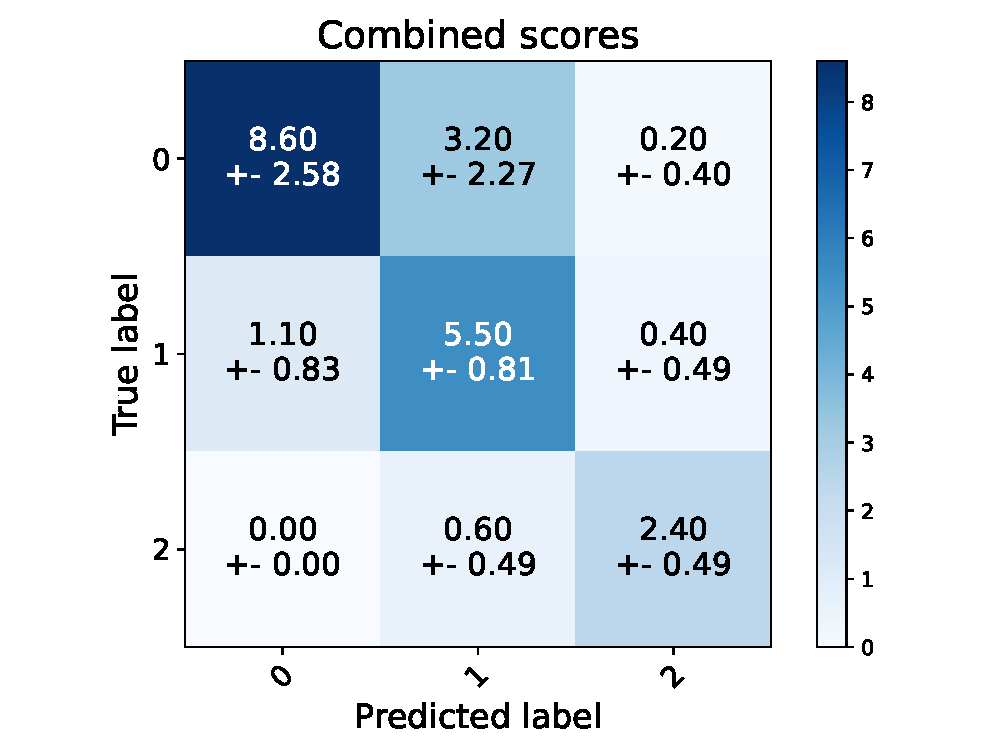
\includegraphics[width=\textwidth]{files/figs/res/trunk/cnf-combined.eps}
      \caption{}
      \label{fig:trunk-cnf-comb}
  \end{subfigure}

  \begin{subfigure}[t]{0.48\textwidth}
      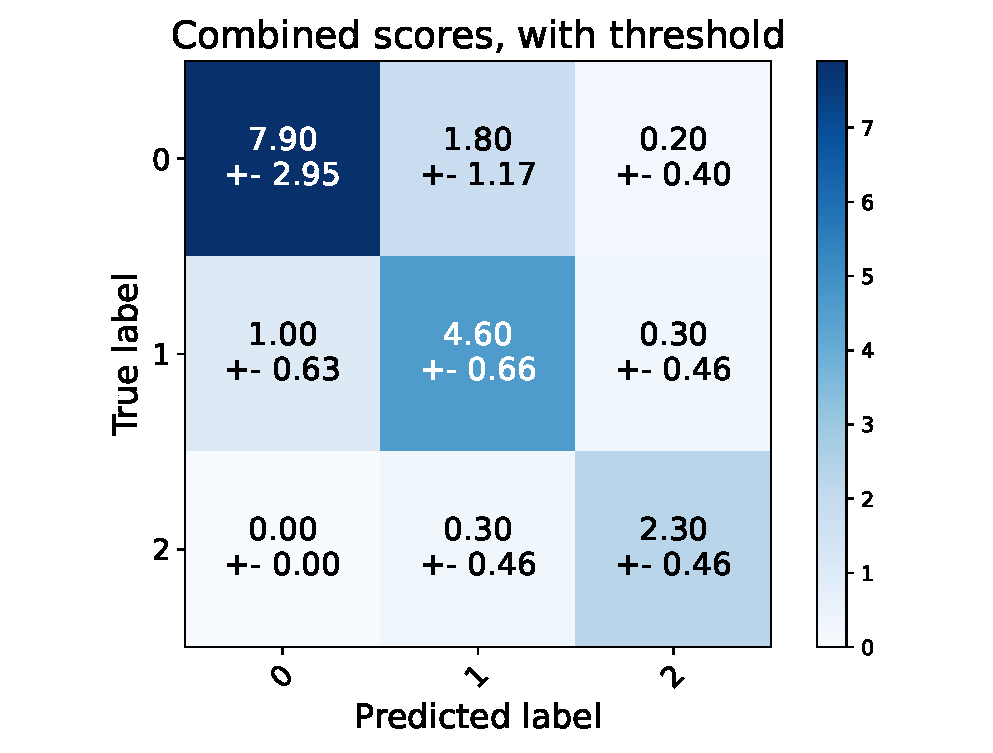
\includegraphics[width=\textwidth]{files/figs/res/trunk/cnf-combined-th.eps}
      \caption{}
      \label{fig:trunk-cnf-comb-th}
  \end{subfigure}
  ~
  \begin{subfigure}[t]{0.48\textwidth}
      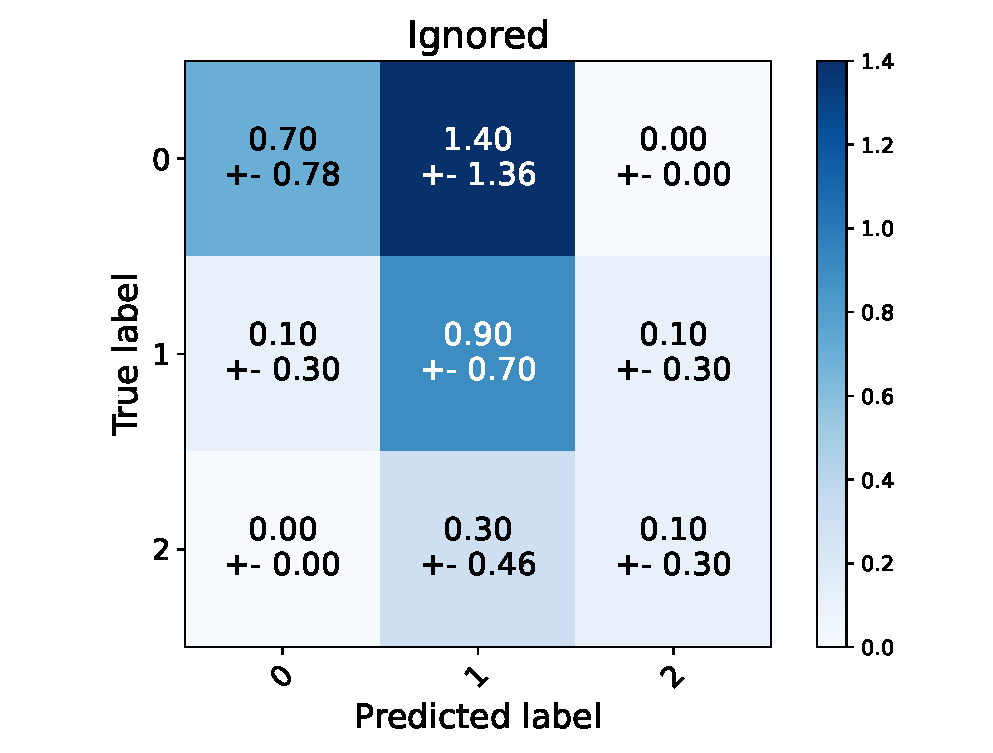
\includegraphics[width=\textwidth]{files/figs/res/trunk/cnf-ignored.eps}
      \caption{}
      \label{fig:trunk-cnf-ignored}
  \end{subfigure}
  \caption{Confusion matrices for the trunk classification on the test set. Classification of the individual repetitions is shown in (a), the combined score for the sequences of 5 repetitions is shown in (b). (c) shows the combined score with the threshold suggested in Section \ref{sec:met-combined}, i.e. all scores with a predicted probability higher than 0.4. The scores ignored due to this threshold are shown in (d). The entries in the matrices show the mean and standard deviation of the 10 ensembles trained in the cross validation.}
  \label{fig:trunk-cnfs}
\end{figure}

\begin{table}[h]
  \caption{The class distribution in the test data for the trunk POE.}
  \label{tab:trunk-class-dist}
  \centering
  \begin{tabu}[c]{cccc}
    \textbf{Class}            & 0, Good & 1, Fair & 2, Poor \\ \hline \hline
    \textbf{Proportion (\%)}  & 47.3 & 38.2 & 14.5
  \end{tabu}
\end{table}


\begin{figure}
  \centering
  \begin{subfigure}[t]{0.4\textwidth}
    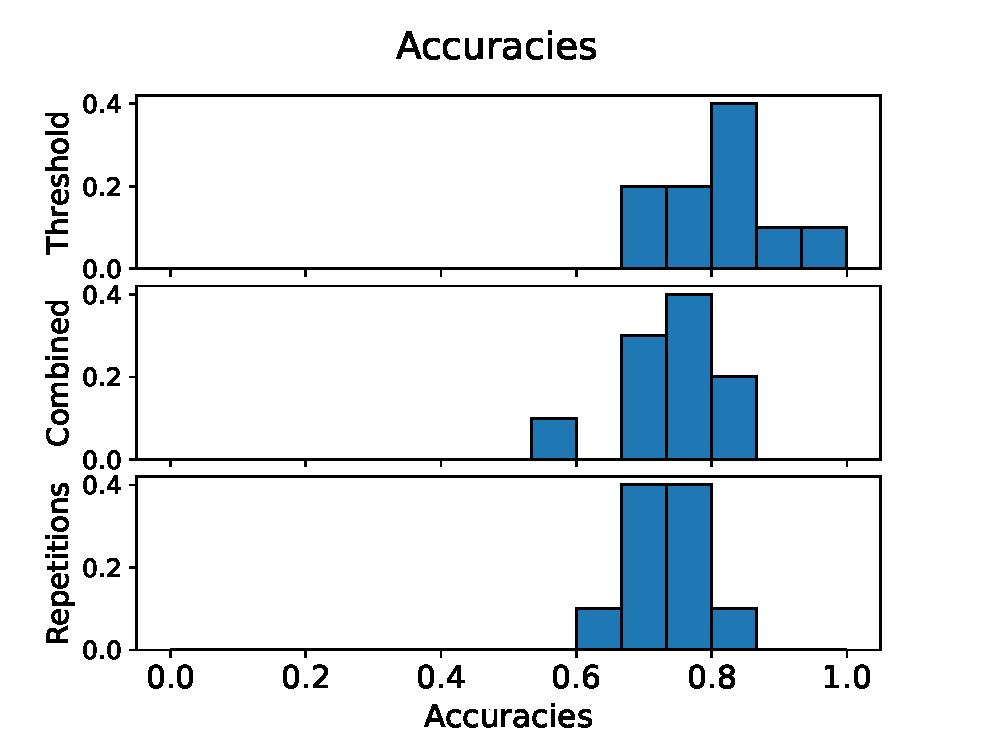
\includegraphics[width=\textwidth]{files/figs/res/trunk/acc.eps}
    \caption{}
    \label{fig:trunk-acc}
  \end{subfigure}
  ~
  \begin{subfigure}[t]{0.4\textwidth}
    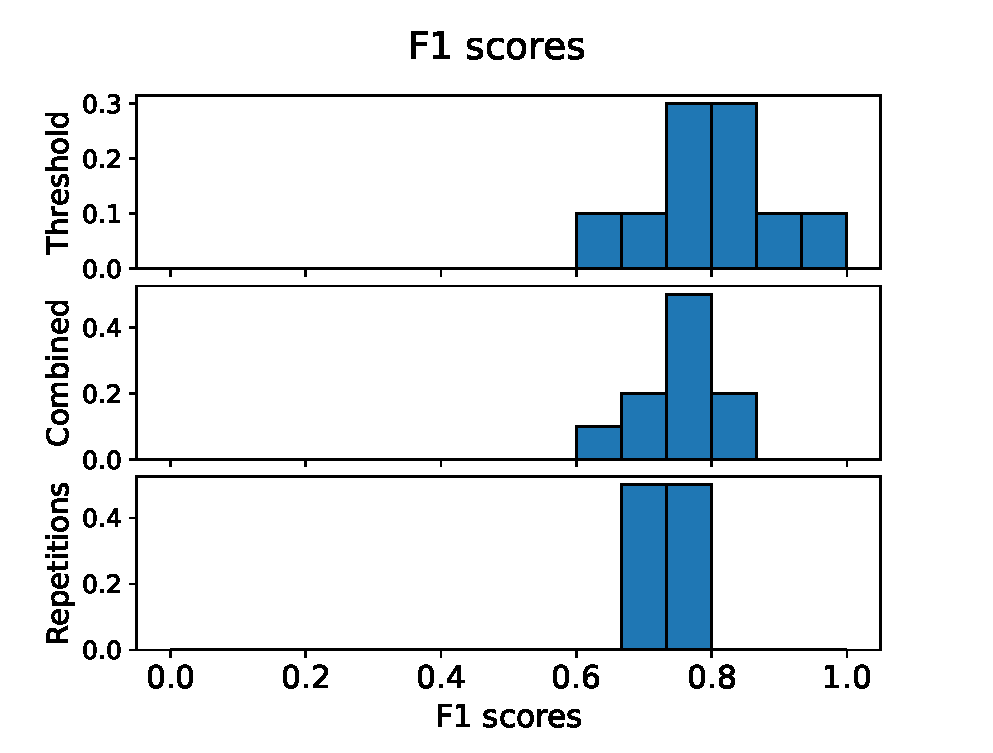
\includegraphics[width=\textwidth]{files/figs/res/trunk/f1.eps}
    \caption{}
    \label{fig:trunk-f1}
  \end{subfigure}

  \begin{subfigure}[t]{0.4\textwidth}
    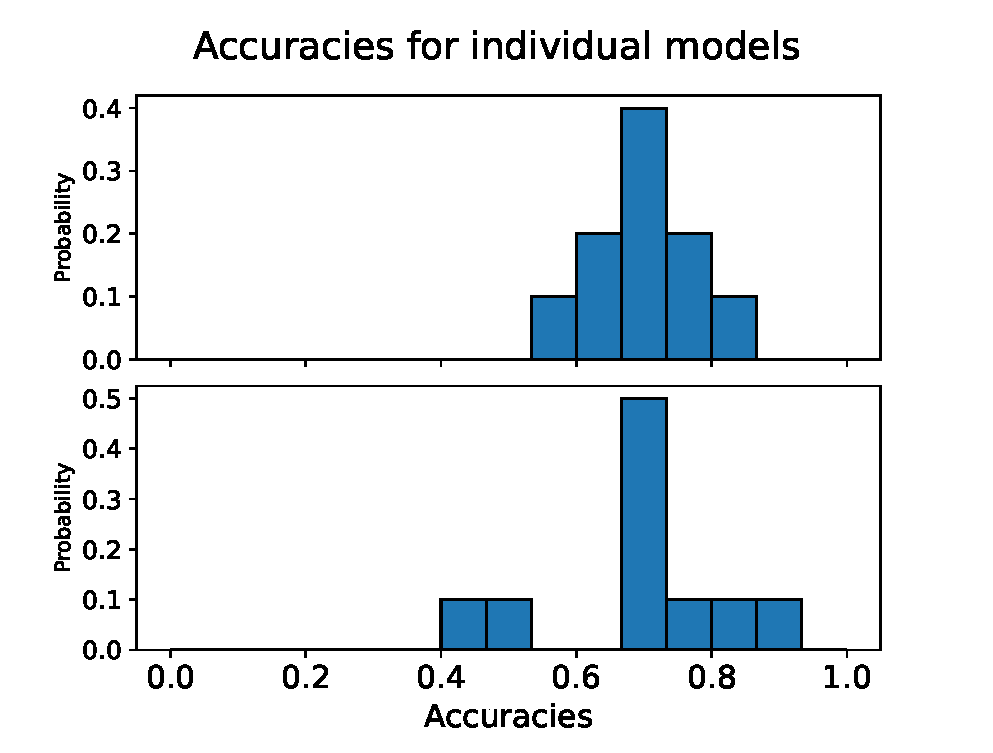
\includegraphics[width=\textwidth]{files/figs/res/trunk/acc-ind.eps}
    \caption{}
    \label{fig:trunk-acc-ind}
  \end{subfigure}
  ~
  \begin{subfigure}[t]{0.4\textwidth}
    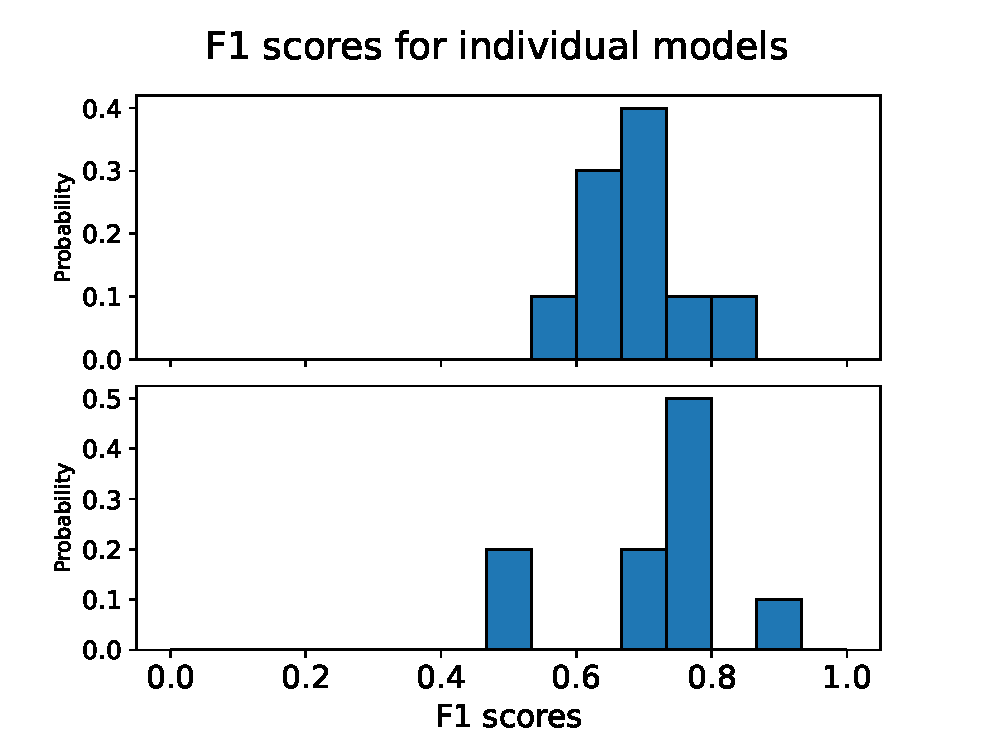
\includegraphics[width=\textwidth]{files/figs/res/trunk/f1-ind.eps}
    \caption{}
    \label{fig:trunk-f1-ind}
  \end{subfigure}
  \caption{Histograms of the accuracies and F1 scores summarized in Table \ref{tab:trunk-results} along with the same metrics for the repetition classification for the models making up the ensembles, presented in Table \ref{tab:ensemble-models}. The high precision models only predicting one class are excluded.}
  \label{fig:trunk-hist-results}
\end{figure}

Based on what is presented in Figures \ref{fig:trunk-cnfs} and \ref{fig:trunk-hist-results} as well as Table \ref{tab:trunk-results}, it seems like the performance of the classifier is enhanced by the measures taken. Table \ref{tab:trunk-improvements} shows this is true with different confidence. Neither the combined score nor the use of an ensemble can be said to improve the performance significantly, but the combined score for the five repetitions is not primarily done to improve the performance, instead this is the way the scoring system is designed. Regarding the ensemble it might be difficult to say how big of an improvement it is based on these metrics, but it reduces the variability in the results. By introducing the threshold, ignoring predictions with a predicted probability lower than 0.4, an average of 3.6 sequences are overlooked. Of these 1.7 were correctly classified and 1.9 were incorrect. %As the compute increases linearly with the number of models used this becomes

From Figure \ref{fig:trunk-cnfs} and Table~\ref{tab:trunk-class-dist} it is clear that the majority of misclassifications are between the classes 0 and 1. This is a natural effect of there being more 0s and 1s than 2s in the test set. Also, asking the experts working with this assessment system these classes are generally the ones difficult to tell apart. Another sign that the model to some extent aligns with the assessments made by the human is the better performance for the sequences where the human expert were certain about the class, seen in Table \ref{tab:trunk-results}.

\begin{table}
  \caption{With what confidence different measures led to improvements, i.e, a higher number means we can be more certain that the performance is increased by performing the corresponding measure. Calculated assuming normal distributions and using pairwise comparisons for the folds. When comparing the ensemble with the individual models the best model is chosen.}
  \label{tab:trunk-improvements}
  \centering
  \begin{tabu}[c]{|c|c|c|c|}
    \hline
    & \multicolumn{1}{c|}{\begin{tabular}[c]{@{}c@{}}\textbf{Ensemble -}\\\textbf{individual} \\\textbf{models}\end{tabular}} &
    \multicolumn{1}{c|}{\begin{tabular}[c]{@{}c@{}}\textbf{Combined -}\\\textbf{Repetitions}\end{tabular}} &
    \multicolumn{1}{c|}{\begin{tabular}[c]{@{}c@{}}\textbf{Threshold -}\\\textbf{Combined}\end{tabular}} \\ \hline
    \textbf{Accuracy} & 85\% & 75\% & 95\% \\ \hline
    \textbf{F1 score} & 75\% & 85\% & 95\% \\ \hline
  \end{tabu}
\end{table}


\begin{figure}
  \centering
  \begin{subfigure}[t]{0.33\textwidth}
    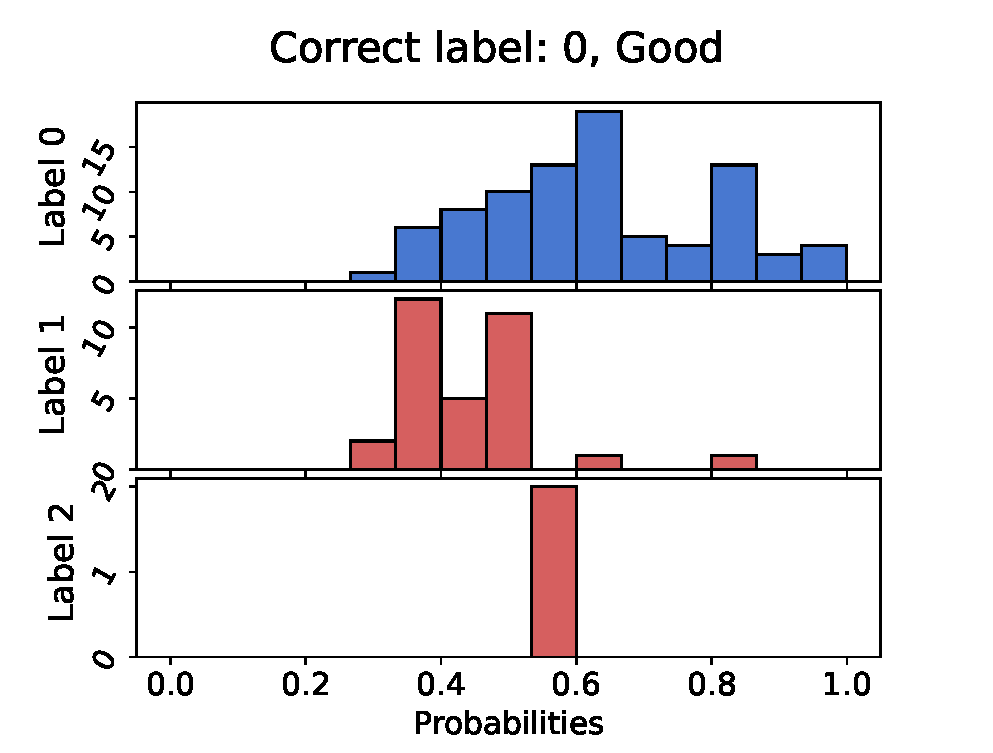
\includegraphics[width=\textwidth]{files/figs/res/trunk/pc0-rb.eps}
    \caption{}
    \label{fig:trunk-pc0}
  \end{subfigure}%
  \begin{subfigure}[t]{0.33\textwidth}
    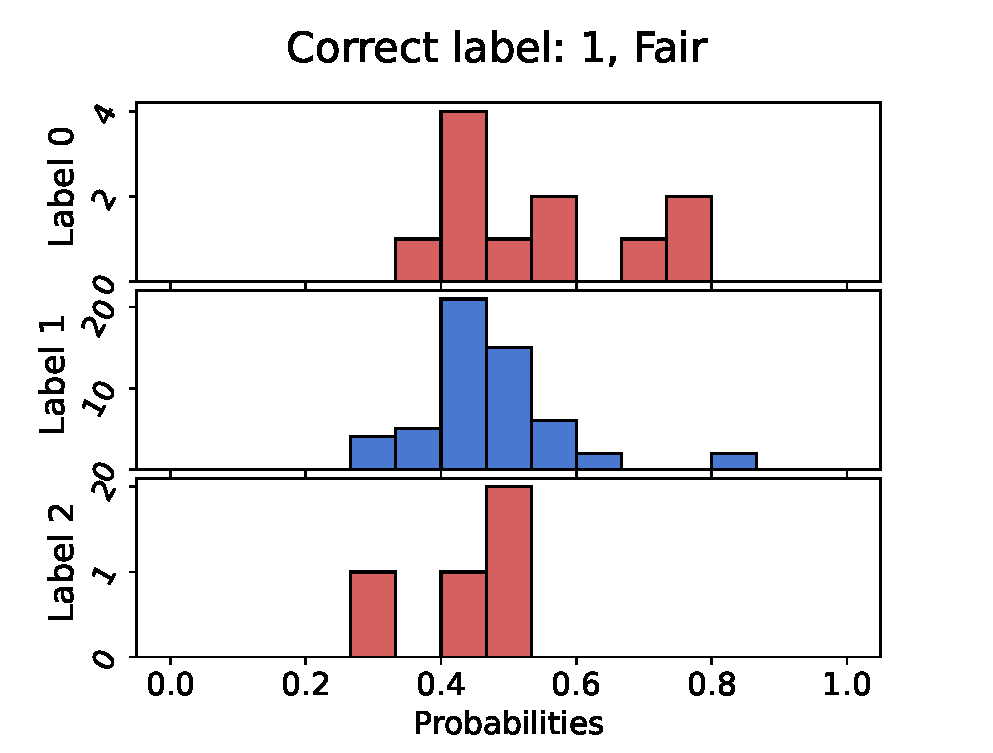
\includegraphics[width=\textwidth]{files/figs/res/trunk/pc1-rb.eps}
    \caption{}
    \label{fig:trunk-pc1}
  \end{subfigure}%
  \begin{subfigure}[t]{0.33\textwidth}
    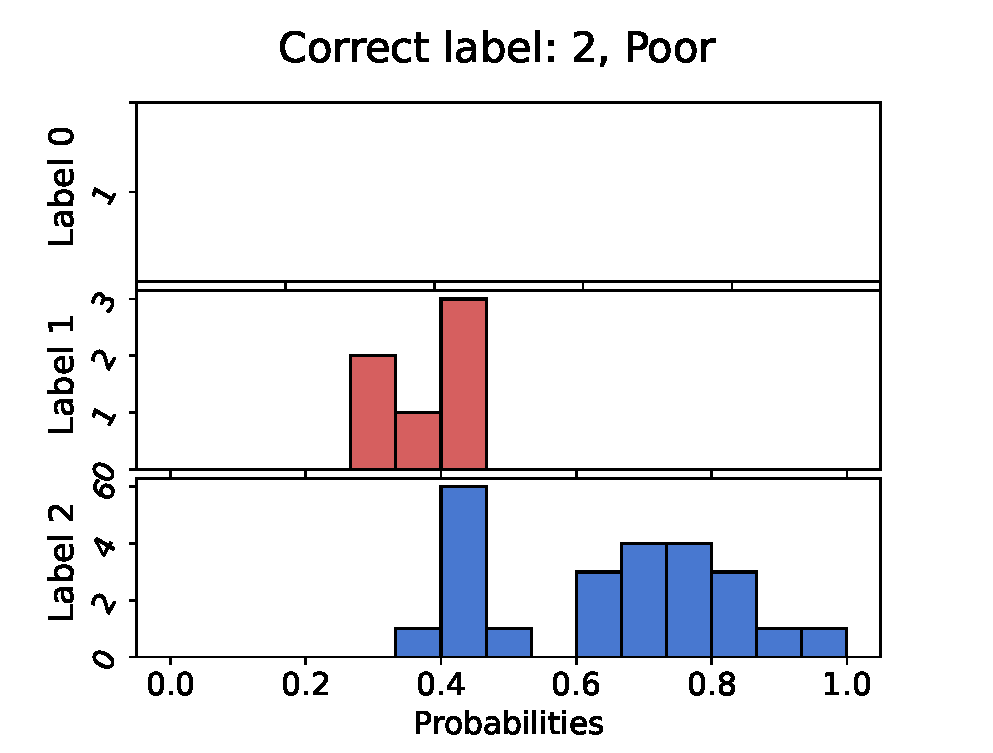
\includegraphics[width=\textwidth]{files/figs/res/trunk/pc2-rb.eps}
    \caption{}
    \label{fig:trunk-pc2}
  \end{subfigure}

  \caption{Figures showing the probabilities for the predicted class, i.e., the argmax of the model output, without threshold, for correct class 0: (a), 1: (b), and 2: (c). Incorrect predictions are shown in red.}
  \label{fig:trunk-pc}
\end{figure}

In the results above, a threshold to ignore uncertain classifications and thereby increase the performance was used. What can be seen as an extension to such a threshold, and something important for clinical use, would be to provide a confidence in the classification. Figure \ref{fig:trunk-pc} shows the probabilities for the predicted class depending on which the correct class actually is. This is the output the threshold acts on, ignoring any sample with a probability lower than 0.4. As suggested in the figure, this measure could be a suitable metric to use as prediction confidence, with the model rarely predicting incorrectly when it outputs a high class probability. However, although the ensemble weights has been adjusted as discussed in Section \ref{sec:met-ensembles}, the probabilities for class 1 is generally low.

\FloatBarrier
\subsection{Pelvis}
As in the previous section, the pelvis results are presented in Table \ref{tab:pelvis-results}, showing the accuracies, F1 scores, recall, and precisions, and in the confusion matrices in Figure \ref{fig:pelvis-cnfs}.
Along with this, histograms showing the effect of the ensemble, combined score, and threshold can be seen in Figure \ref{fig:pelvis-hist-results} and these effects are also summarized in Table \ref{tab:pelvis-improvements}. The class distribution in the test set is presented in Table~\ref{tab:pelvis-class-dist}.

\begin{table}[h]
  \centering
  \caption{Results of the ensemble for the pelvis POE. Rep., Comb., and Thresh. represents the results for the repetitions, combinations, and combinations with thresholds, respectively. The Certainties columns show the results making up the Comb. column, but for the certainty levels of the expert labeling the data. These ranges from certain (0) to uncertain (2), the variable $n$ shows how many datapoints each category contains. All results are the mean from the 10 folds $\pm$ the corresponding standard deviations. F1, recall, and precision are macro averaged.}
  \label{tab:pelvis-results}
  \small
  \begin{tabu}[c]{|c|c|c|c||c|c|c|}
    \hline
    % & \multirow21}{*}{Repetitions} & \multirow{2}{*}{Combinations} & \multirow{2}{*}{Thresholds} &  \multirow{2}{*}\multicolumn{3}{c}{Certainties}\\
    & \multirow{2}{*}{\textbf{Rep.}} & \multirow{2}{*}{\textbf{Comb.}} & \multirow{2}{*}{\textbf{Thresh.}} & \multicolumn{3}{c|}{\textbf{Certainties}}\\ \cline{5-7}
    & & & &0($n$=14)&1($n$=7)&2($n$=1)\\ \hline
    Accuracy (\%)   &63.6$\pm$10.7&69.1$\pm$10.1&\textbf{73.3$\pm$18.9}&
                    67.9$\pm$15.0&70.0$\pm$19.6&\textbf{80.0$\pm$40.0}\\ \hline
    F1 score (\%)   &55.7$\pm$13.4&66.5$\pm$15.0&\textbf{73.6$\pm$22.3}&
                    58.0$\pm$20.1&\textbf{63.7$\pm$23.8}&31.7$\pm$17.4\\ \hline
    Recall (\%)     &57.3$\pm$12.0&75.3$\pm$14.0&\textbf{77.9$\pm$14.9}&
                    56.8$\pm$20.7&\textbf{64.6$\pm$22.8}&31.7$\pm$17.4\\ \hline
    Precision (\%)  &58.3$\pm$14.9&67.0$\pm$14.4&\textbf{74.9$\pm$23.8}&
                    62.5$\pm$19.7&\textbf{68.4$\pm$24.0}&31.7$\pm$17.4\\ \hline
  \end{tabu}
\end{table}

Overall it is clear that the performance is worse for the pelvis as compared to the other \glspl{poe}. Although the different scores are not that much lower compared to the trunk \gls{poe} they vary much more making it difficult to draw any conclusions from it. It also looks less like a normal distribution, making Table \ref{tab:pelvis-improvements} unreliable. One explanation for this behavior is that the human experts considers this \gls{poe} to be the most difficult one to assess of the four considered in work. The reason for this is that the hip rotates in several planes making it difficult to assess in 2D. This probably affects the models, both directly as a more difficult pattern to identify, which might rely on information not available in this 2D data. It might also affect the models indirectly as this suggests that the training labels can be more unreliable. The higher uncertainty can also be seen in Figure \ref{fig:pelvis-cnf-ignored} as more sequences are ignored due to the threshold, 7.6 on average in this case. The high number of ignored samples is one explanation for the higher variance in the different metrics after applying the threshold.

\begin{figure}[h]
  \centering
  \begin{subfigure}[t]{0.48\textwidth}
      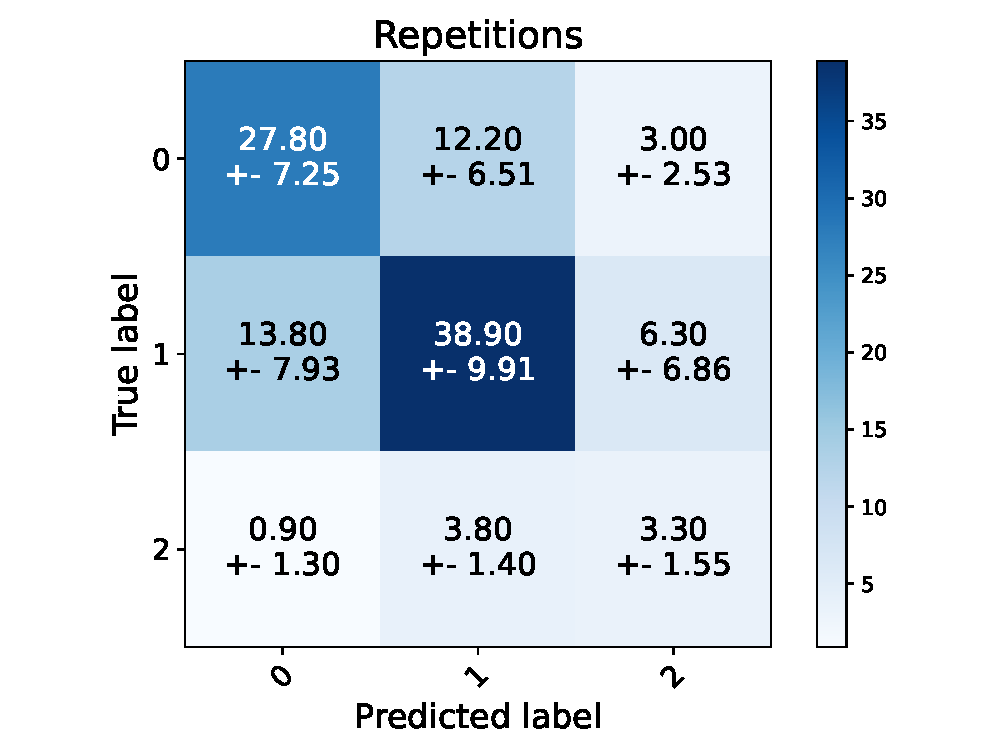
\includegraphics[width=\textwidth]{files/figs/res/pelvis/cnf-reps.eps}
      \caption{}
      \label{fig:pelvis-cnf-reps}
  \end{subfigure}
  ~
  \begin{subfigure}[t]{0.48\textwidth}
      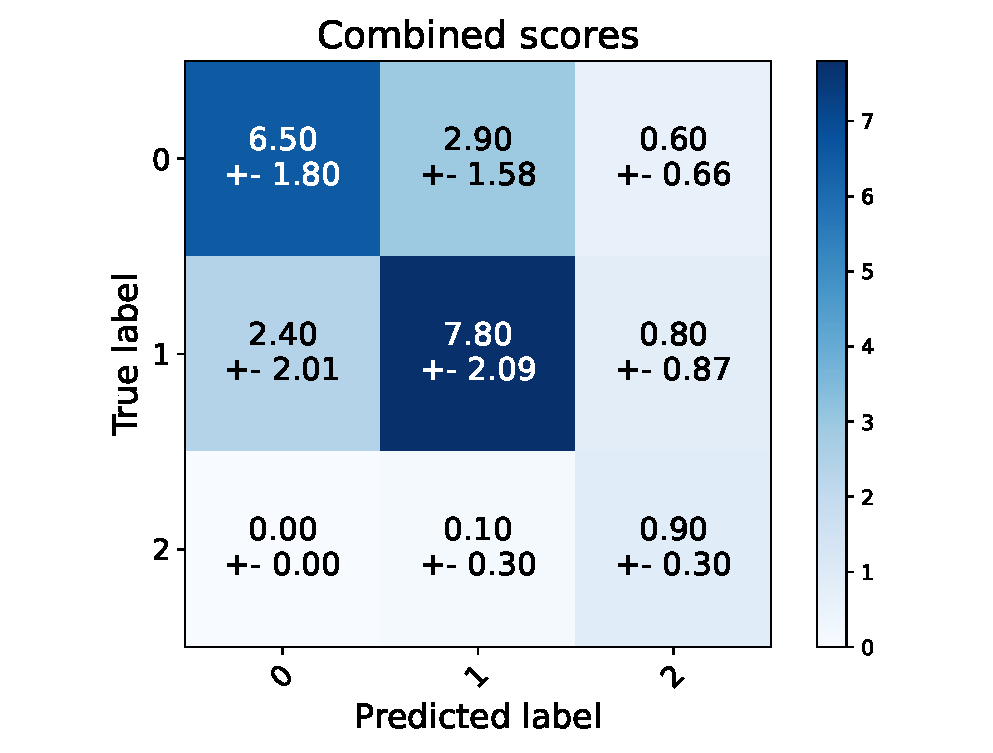
\includegraphics[width=\textwidth]{files/figs/res/pelvis/cnf-combined.eps}
      \caption{}
      \label{fig:pelvis-cnf-comb}
  \end{subfigure}

  \begin{subfigure}[t]{0.48\textwidth}
      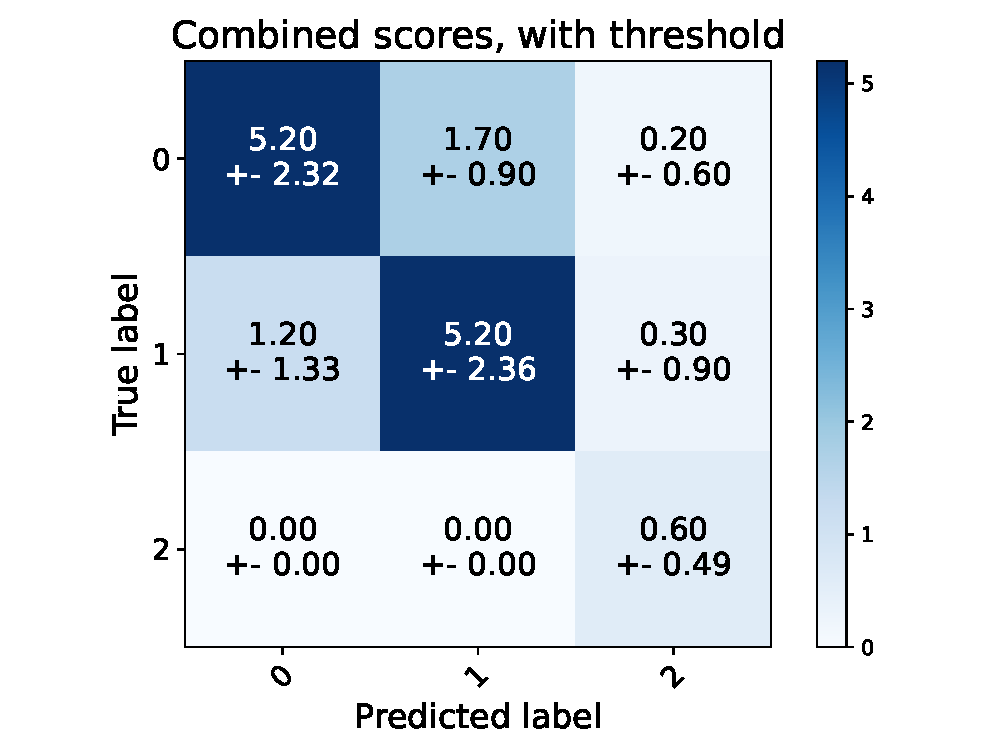
\includegraphics[width=\textwidth]{files/figs/res/pelvis/cnf-combined-th.eps}
      \caption{}
      \label{fig:pelvis-cnf-comb-th}
  \end{subfigure}
  ~
  \begin{subfigure}[t]{0.48\textwidth}
      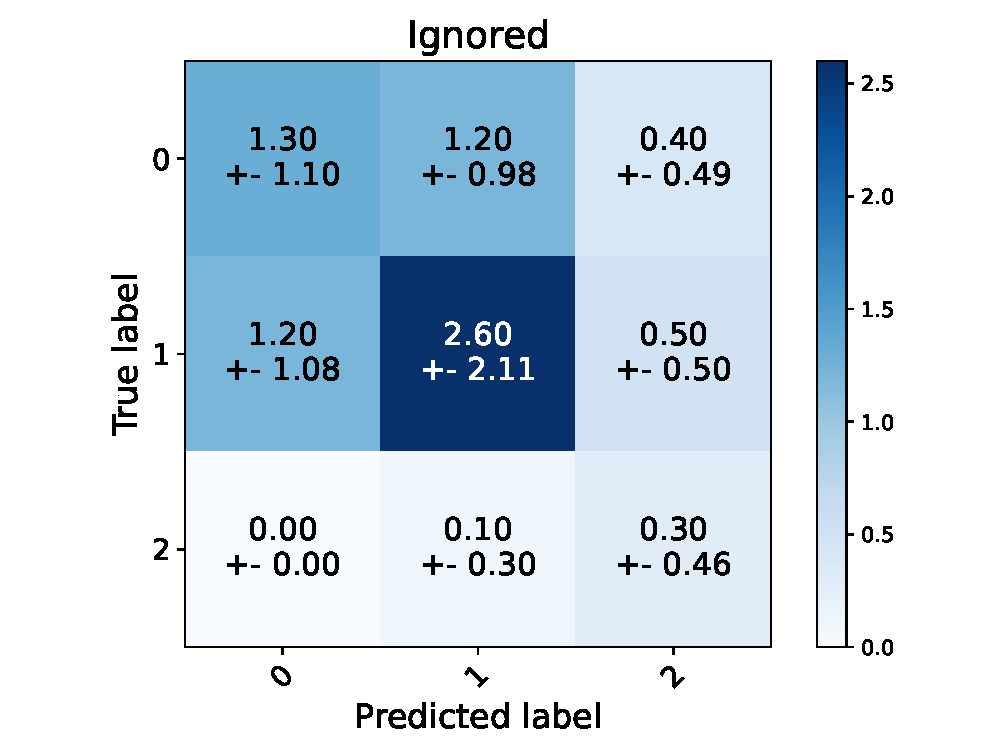
\includegraphics[width=\textwidth]{files/figs/res/pelvis/cnf-ignored.eps}
      \caption{}
      \label{fig:pelvis-cnf-ignored}
  \end{subfigure}
  \caption{Confusion matrices for the pelvis classification on the test set. Classification of the individual repetitions is shown in (a), the combined score for the sequences of 5 repetitions is shown in (b). (c) shows the combined score with the threshold suggested in Section \ref{sec:met-combined}, i.e. all scores with a predicted probability higher than 0.4. The scores ignored due to this threshold are shown in (d). The entries in the matrices show the mean and standard deviation of the 10 ensembles trained in the cross validation.}
  \label{fig:pelvis-cnfs}
\end{figure}

\begin{table}[h]
  \caption{The class distribution in the test data for the pelvis POE.}
  \label{tab:pelvis-class-dist}
  \centering
  \begin{tabu}[c]{cccc}
    \textbf{Class}            & 0, Good & 1, Fair & 2, Poor \\ \hline \hline
    \textbf{Proportion (\%)}  & 39.1 & 53.6 & 7.3
  \end{tabu}
\end{table}

\begin{figure}
  \centering
  \begin{subfigure}[t]{0.4\textwidth}
    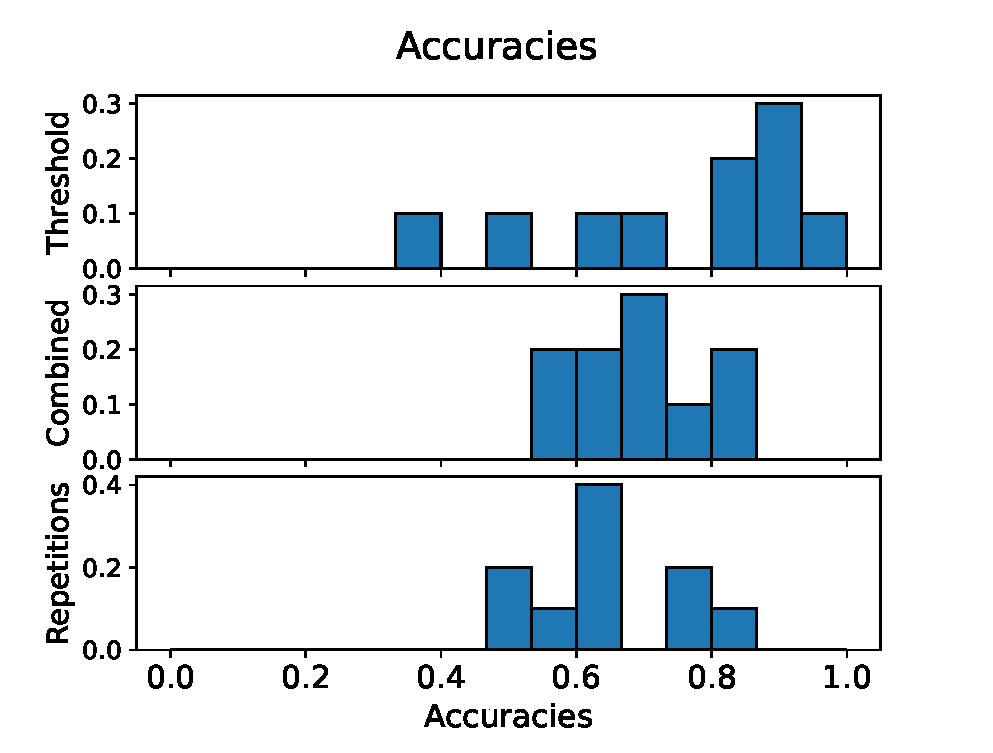
\includegraphics[width=\textwidth]{files/figs/res/pelvis/acc.eps}
    \caption{}
    \label{fig:pelvis-acc}
  \end{subfigure}
  ~
  \begin{subfigure}[t]{0.4\textwidth}
    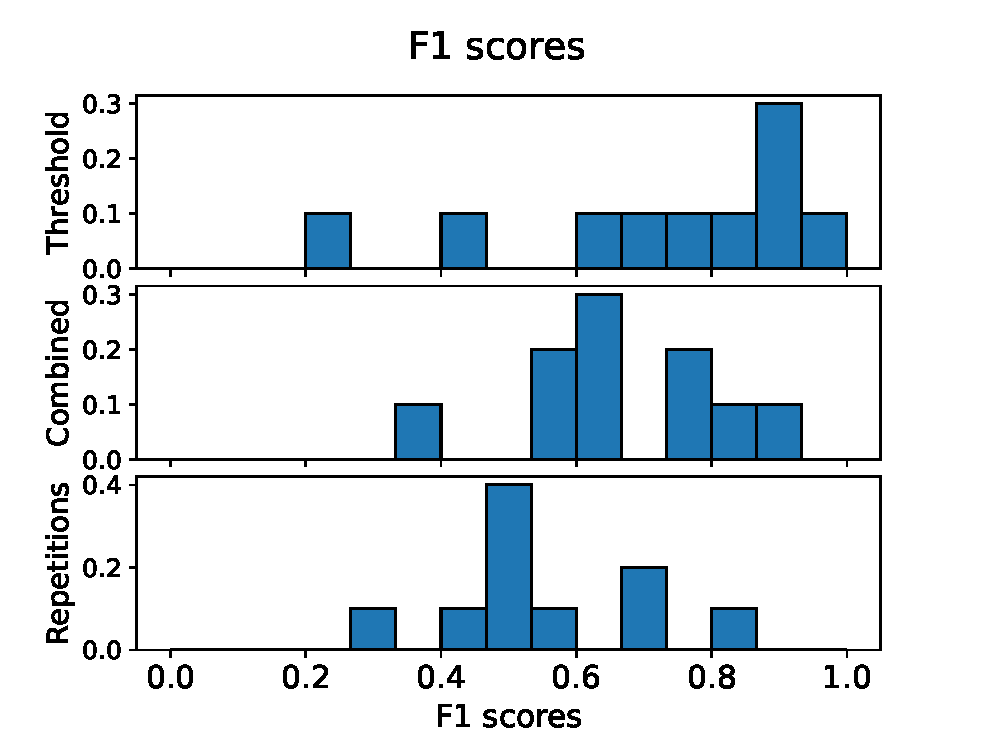
\includegraphics[width=\textwidth]{files/figs/res/pelvis/f1.eps}
    \caption{}
    \label{fig:pelvis-f1}
  \end{subfigure}

  \begin{subfigure}[t]{0.4\textwidth}
    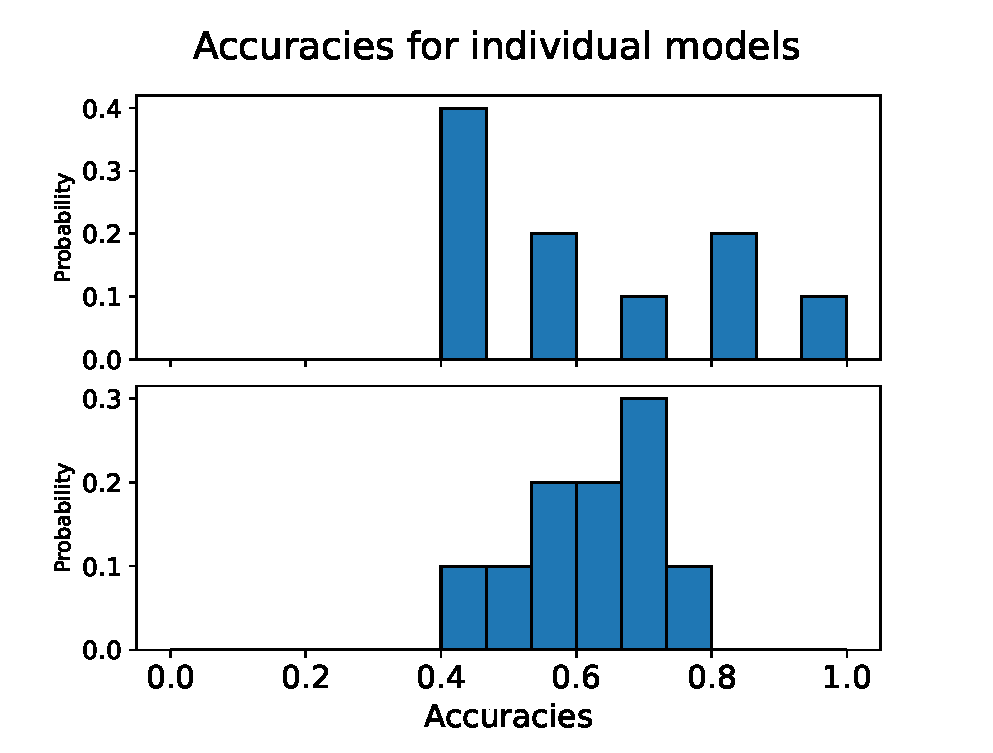
\includegraphics[width=\textwidth]{files/figs/res/pelvis/acc-ind.eps}
    \caption{}
    \label{fig:pelvis-acc-ind}
  \end{subfigure}
  ~
  \begin{subfigure}[t]{0.4\textwidth}
    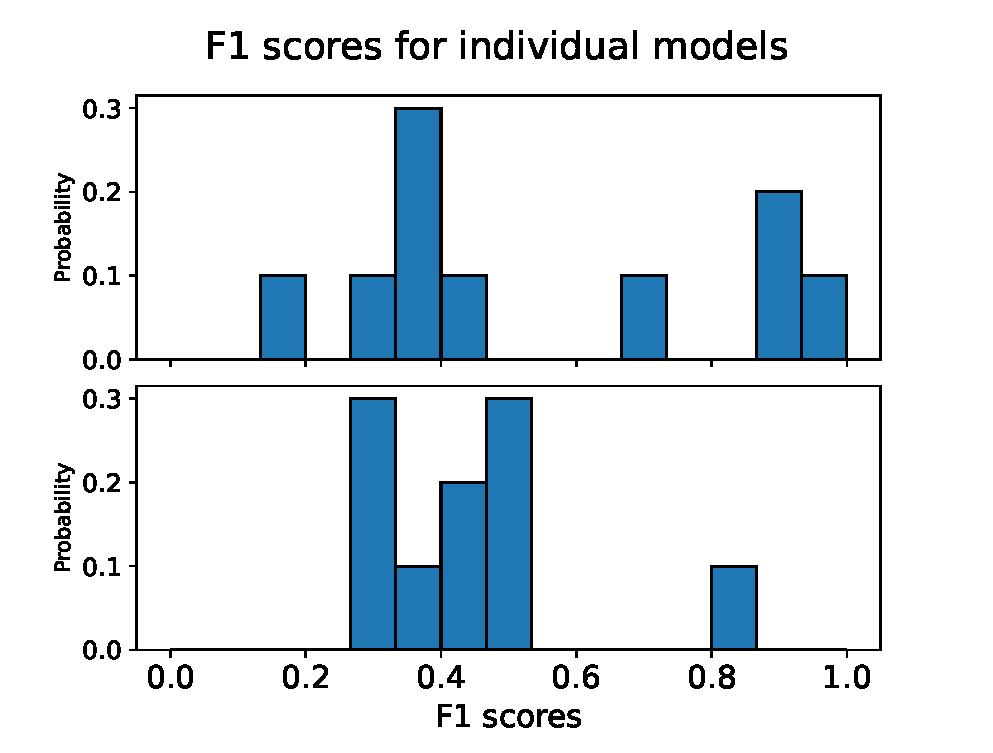
\includegraphics[width=\textwidth]{files/figs/res/pelvis/f1-ind.eps}
    \caption{}
    \label{fig:pelvis-f1-ind}
  \end{subfigure}
  \caption{Histograms of the accuracies and F1 scores summarized in Table \ref{tab:pelvis-results} along with the same metrics for the repetition classification for the models making up the ensembles, presented in Table \ref{tab:ensemble-models}. The high precision models only predicting one class are excluded.}
  \label{fig:pelvis-hist-results}
\end{figure}

\begin{table}
  \caption{With what confidence different measures led to improvements, i.e, a higher number means we can be more certain that the performance is increased by performing the corresponding measure. Calculated assuming normal distributions and using pairwise comparisons for the folds. When comparing the ensemble with the individual models the best model is chosen.}
  \label{tab:pelvis-improvements}
  \centering
  \begin{tabu}[c]{|c|c|c|c|}
    \hline
    & \multicolumn{1}{c|}{\begin{tabular}[c]{@{}c@{}}\textbf{Ensemble -}\\\textbf{individual} \\\textbf{models}\end{tabular}} &
    \multicolumn{1}{c|}{\begin{tabular}[c]{@{}c@{}}\textbf{Combined -}\\\textbf{Repetitions}\end{tabular}} &
    \multicolumn{1}{c|}{\begin{tabular}[c]{@{}c@{}}\textbf{Threshold -}\\\textbf{Combined}\end{tabular}} \\ \hline
    \textbf{Accuracy} & - & 95\% & 85\% \\ \hline
    \textbf{F1 score} & - & 95\% & 95\% \\ \hline
  \end{tabu}
\end{table}


\begin{figure}
  \centering
  \begin{subfigure}[t]{0.33\textwidth}
    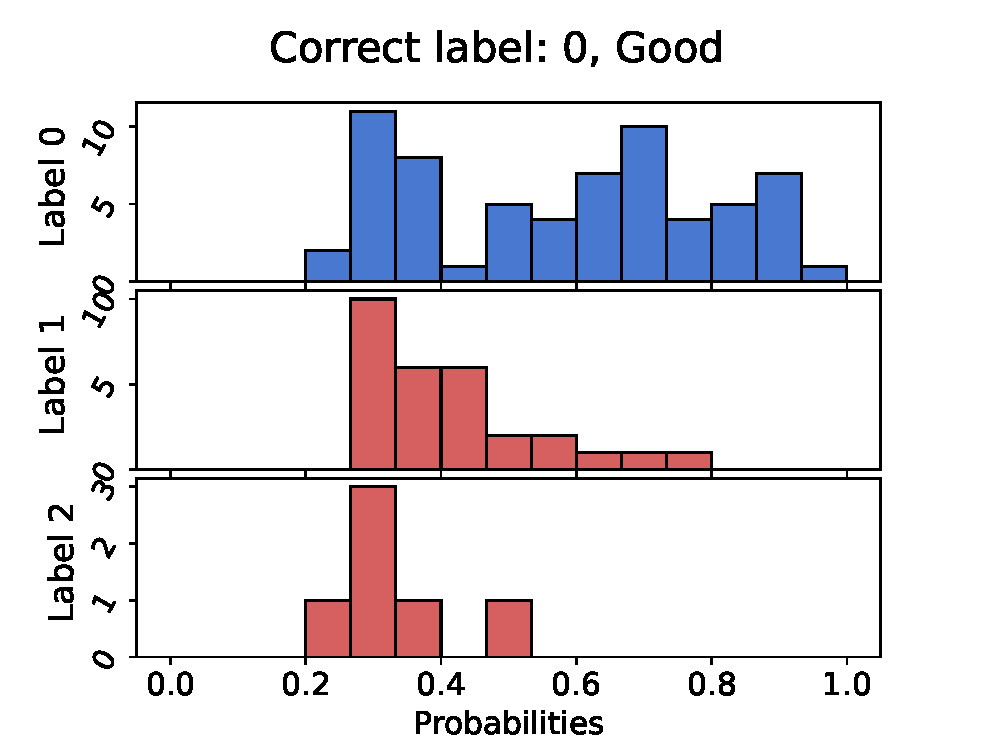
\includegraphics[width=\textwidth]{files/figs/res/pelvis/pc0-rb.eps}
    \caption{}
    \label{fig:pelvis-pc0}
  \end{subfigure}%
  \begin{subfigure}[t]{0.33\textwidth}
    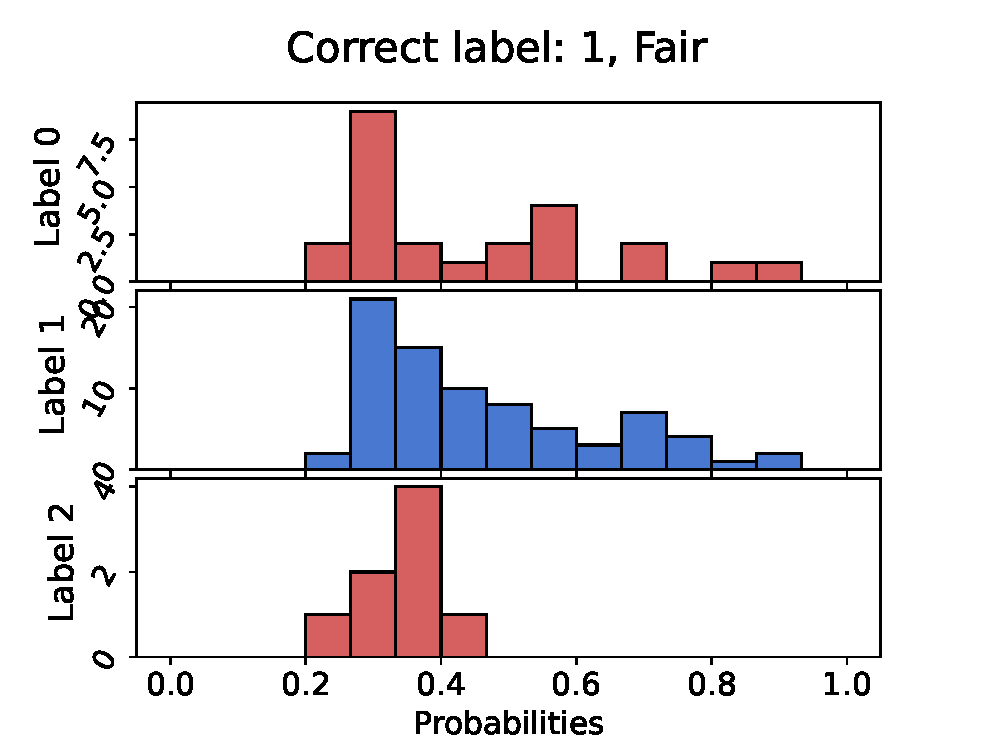
\includegraphics[width=\textwidth]{files/figs/res/pelvis/pc1-rb.eps}
    \caption{}
    \label{fig:pelvis-pc1}
  \end{subfigure}%
  \begin{subfigure}[t]{0.33\textwidth}
    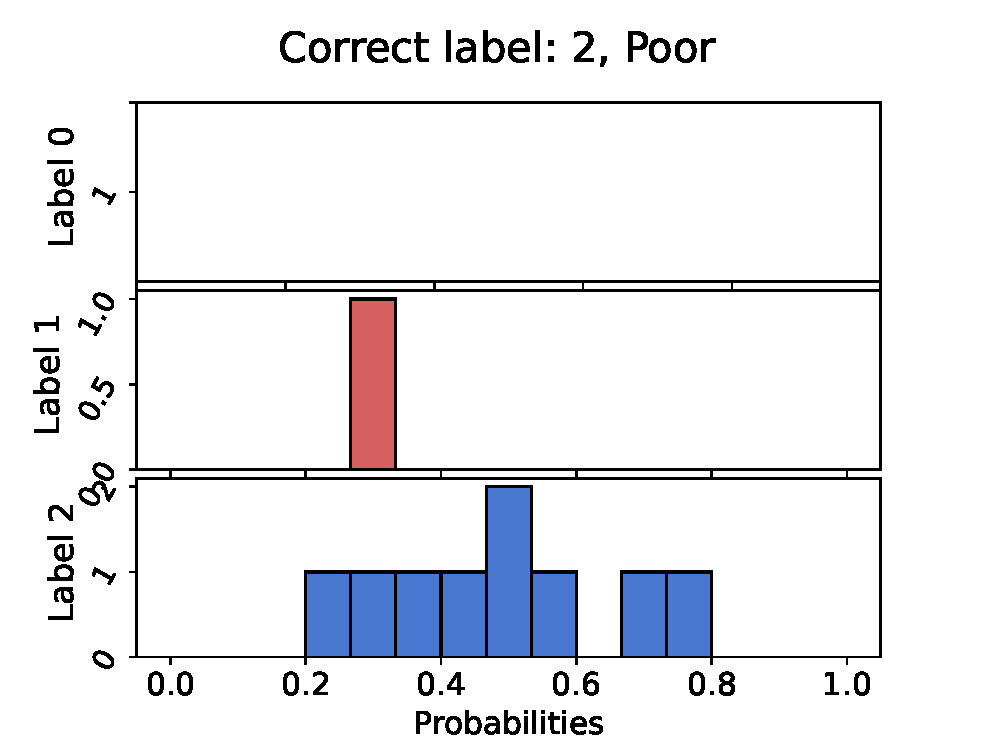
\includegraphics[width=\textwidth]{files/figs/res/pelvis/pc2-rb.eps}
    \caption{}
    \label{fig:pelvis-pc2}
  \end{subfigure}

  \caption{Figures showing the probabilities for the predicted class, i.e., the argmax of the model output, without threshold, for correct class 0: (a), 1: (b), and 2: (c). Incorrect predictions are shown in red.}
  \label{fig:pelvis-pc}
\end{figure}


\FloatBarrier
\subsection{Femoral Valgus}
The results for the femoral valgus \gls{poe} can be found in Figures \ref{fig:femval-cnfs}, \ref{fig:femval-hist-results}, and \ref{fig:femval-pc} as well as in Tables \ref{tab:femval-results} and \ref{tab:femval-improvements}.
This model performs well, but it seems to be slightly biased, at least for this data, towards class 1. To some extent, this can be explained by the class distribution, found in Table~\ref{tab:femval-class-dist}. On average 2.2 samples are ignored because of the threshold and 1.1 of these were correct. Notable is that it classifies a class 2 as a 0 three times and none of these are ignored due to the threshold. As can be seen in Figure~\ref{fig:femval-pc}, two of these have a probability right above the threshold of 0.4.

\begin{table}[h]
  \centering
  \caption{Results of the ensemble for the femoral valgus POE. Rep., Comb., and Thresh. represents the results for the repetitions, combinations, and combinations with thresholds, respectively. The Certainties columns show the results making up the Comb. column, but for the certainty levels of the expert labeling the data. These ranges from certain (0) to uncertain (2), the variable $n$ shows how many datapoints each category contains. All results are the mean from the 10 folds $\pm$ the corresponding standard deviations. F1, recall, and precision are macro averaged.}
  \label{tab:femval-results}
  \small
    \begin{tabu}[c]{|c|c|c|c||c|c|c|}
      \hline
      & \multirow{2}{*}{\textbf{Rep.}} & \multirow{2}{*}{\textbf{Comb.}} & \multirow{2}{*}{\textbf{Thresh.}} & \multicolumn{3}{c|}{\textbf{Certainties}}\\ \cline{5-7}
      & & & &0($n$=15)&1($n$=7)&2($n$=0)\\ \hline
      Accuracy (\%)   &69.6$\pm$6.8&79.1$\pm$9.3&\textbf{82.3$\pm$6.0}&\textbf{82.7$\pm$9.5}&71.4$\pm$11.0&-\\ \hline
      F1 score (\%)   &69.0$\pm$6.6&77.6$\pm$8.6&\textbf{81.0$\pm$5.2}&\textbf{80.8$\pm$8.6}&70.1$\pm$9.4&-\\ \hline
      Recall (\%)     &68.4$\pm$6.3&76.3$\pm$8.1&\textbf{79.5$\pm$5.5}&\textbf{80.4$\pm$7.4}&71.1$\pm$9.5&-\\ \hline
      Precision (\%)  &74.0$\pm$7.4&83.8$\pm$7.4&\textbf{86.5$\pm$5.6}&\textbf{85.2$\pm$7.6}&81.8$\pm$6.6&-\\ \hline
    \end{tabu}
\end{table}

Clearly, the performance is improved by the calculating the combined score and applying the threshold. For this \gls{poe}, the variance is also decreased by introducing the threshold, which was not the case for trunk, pelvis, nor \gls{kmfp}. As can be seen in Table~\ref{tab:femval-improvements}, the ensemble is not improving the performance, but it gives a more robust model neglecting the poor performance which can be seen in Figures \ref{fig:femval-acc-ind} and \ref{fig:femval-f1-ind} for the individual models for one of the folds.

\begin{table}[H]
  \caption{The class distribution in the test data for the femoral valgus POE.}
  \label{tab:femval-class-dist}
  \centering
  \begin{tabu}[c]{cccc}
    \textbf{Class}            & 0, Good & 1, Fair & 2, Poor \\ \hline \hline
    \textbf{Proportion (\%)}  & 32.7 & 40.0 & 27.3
  \end{tabu}
\end{table}

\begin{figure}[H]
  \centering
  \begin{subfigure}[t]{0.48\textwidth}
      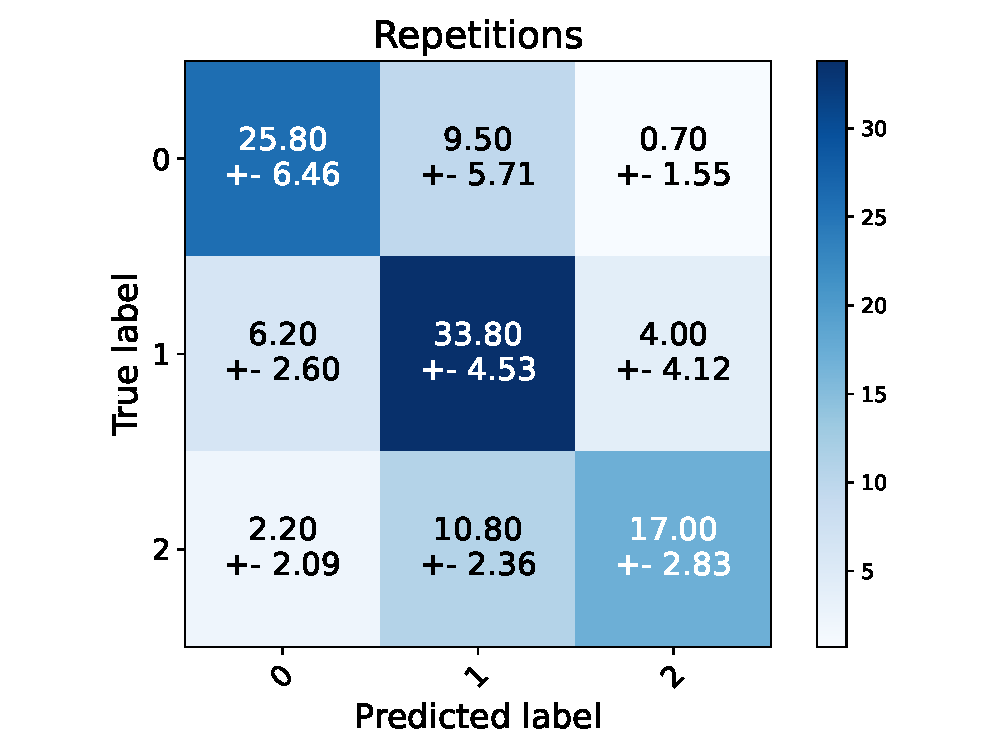
\includegraphics[width=\textwidth]{files/figs/res/femval/cnf-reps.eps}
      \caption{}
      \label{fig:femval-cnf-reps}
  \end{subfigure}
  ~
  \begin{subfigure}[t]{0.48\textwidth}
      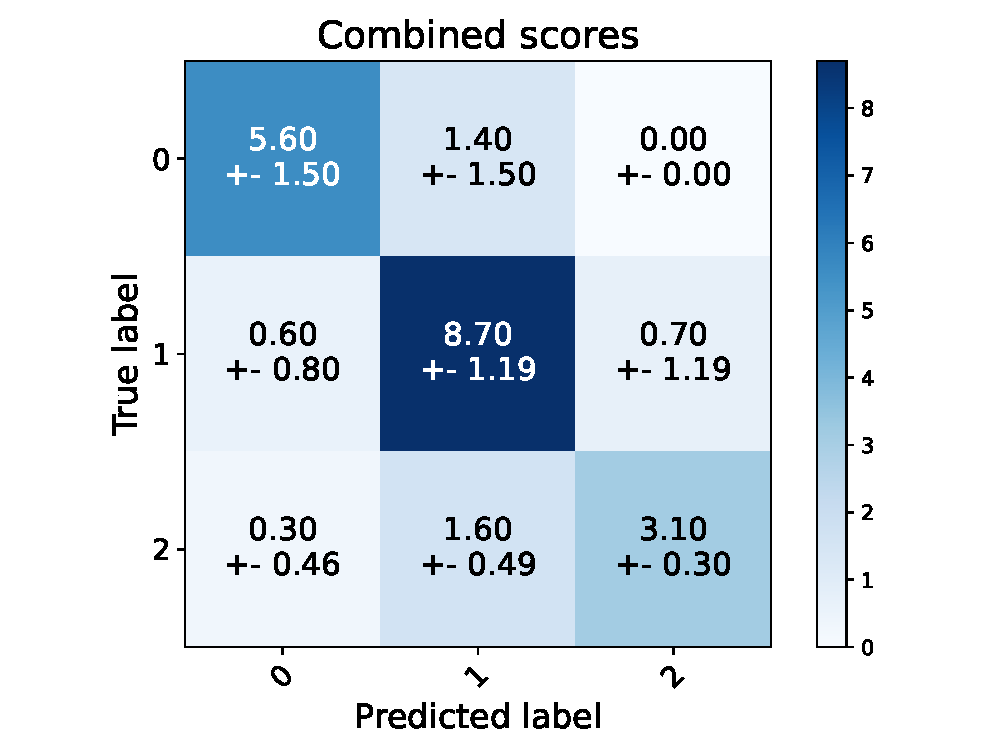
\includegraphics[width=\textwidth]{files/figs/res/femval/cnf-combined.eps}
      \caption{}
      \label{fig:femval-cnf-comb}
  \end{subfigure}

  \begin{subfigure}[t]{0.48\textwidth}
      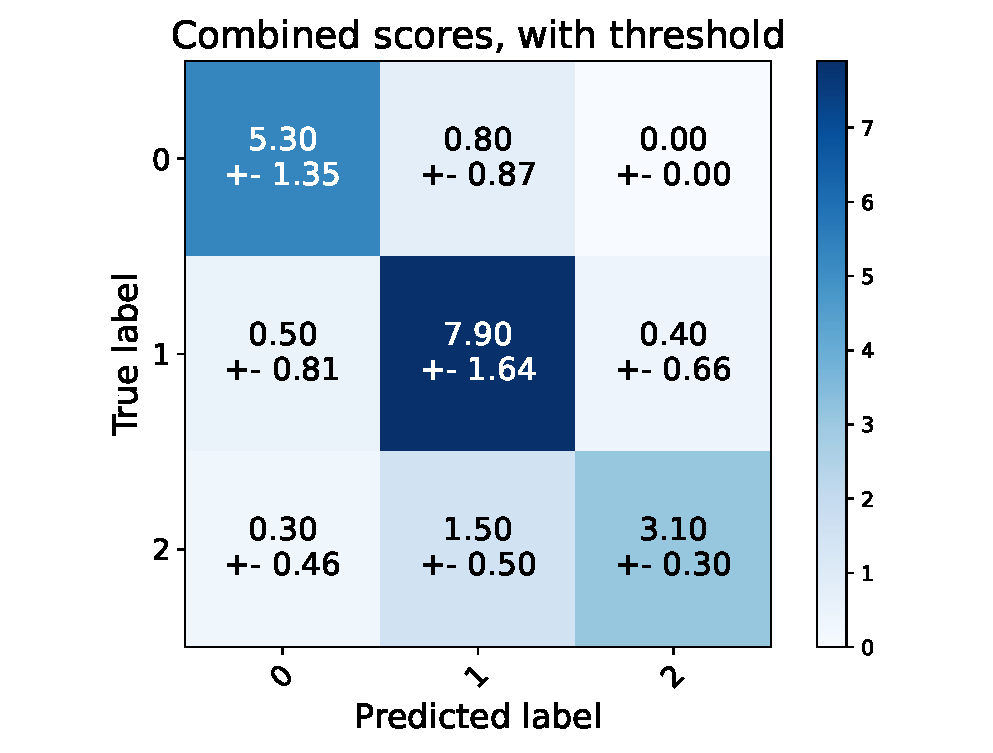
\includegraphics[width=\textwidth]{files/figs/res/femval/cnf-combined-th.eps}
      \caption{}
      \label{fig:femval-cnf-comb-th}
  \end{subfigure}
  ~
  \begin{subfigure}[t]{0.48\textwidth}
      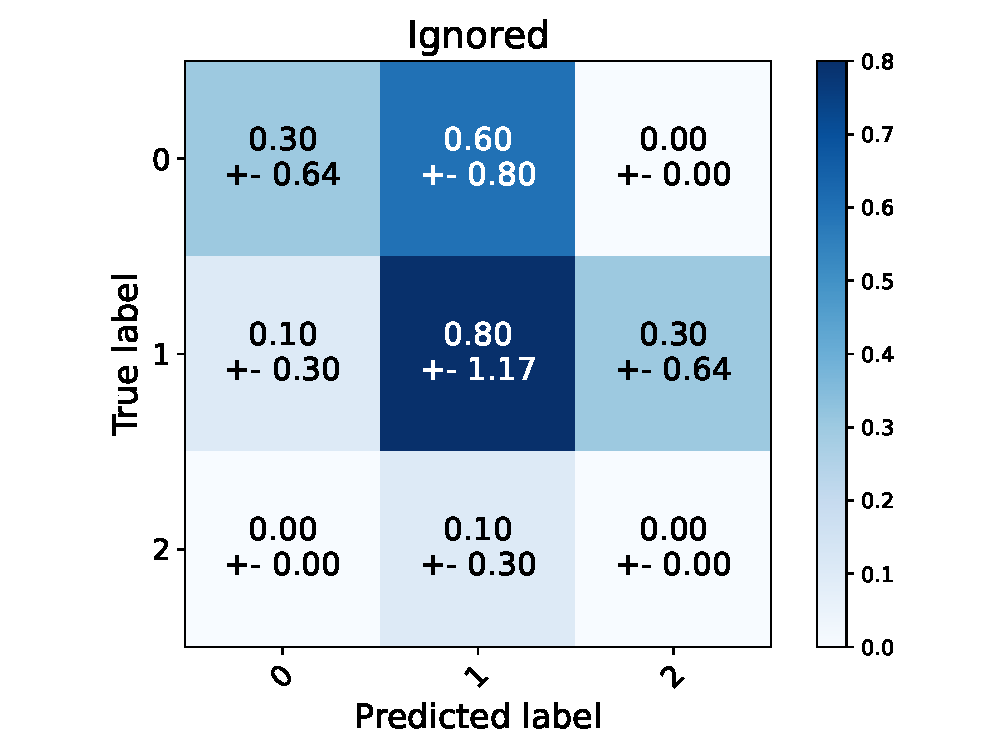
\includegraphics[width=\textwidth]{files/figs/res/femval/cnf-ignored.eps}
      \caption{}
      \label{fig:femval-cnf-ignored}
  \end{subfigure}
  \caption{Confusion matrices for the femoral valgus classification on the test set. Classification of the individual repetitions is shown in (a), the combined score for the sequences of 5 repetitions is shown in (b). (c) shows the combined score with the threshold suggested in Section \ref{sec:met-combined}, i.e. all scores with a predicted probability higher than 0.4. The scores ignored due to this threshold are shown in (d). The entries in the matrices show the mean and standard deviation of the 10 ensembles trained in the cross validation.}
  \label{fig:femval-cnfs}
\end{figure}

\begin{table}[h]
  \caption{With what confidence different measures led to improvements, i.e, a higher number means we can be more certain that the performance is increased by performing the corresponding measure. Calculated assuming normal distributions and using pairwise comparisons for the folds. When comparing the ensemble with the individual models the best model is chosen.}
  \label{tab:femval-improvements}
  \centering
  \begin{tabu}[c]{|c|c|c|c|}
    \hline
    & \multicolumn{1}{c|}{\begin{tabular}[c]{@{}c@{}}\textbf{Ensemble -}\\\textbf{individual} \\\textbf{models}\end{tabular}} &
    \multicolumn{1}{c|}{\begin{tabular}[c]{@{}c@{}}\textbf{Combined -}\\\textbf{Repetitions}\end{tabular}} &
    \multicolumn{1}{c|}{\begin{tabular}[c]{@{}c@{}}\textbf{Threshold -}\\\textbf{Combined}\end{tabular}} \\ \hline
    \textbf{Accuracy} & - & 95\% & 95\% \\ \hline
    \textbf{F1 score} & - & 95\% & 95\% \\ \hline
  \end{tabu}
\end{table}

\begin{figure}
  \centering
  \begin{subfigure}[t]{0.4\textwidth}
    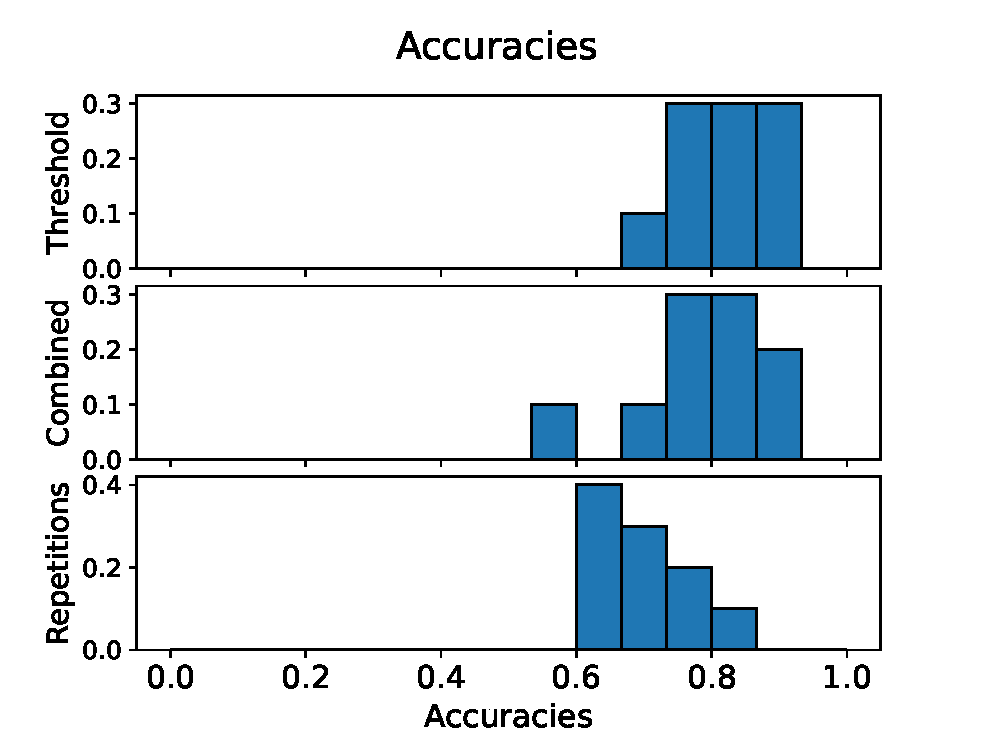
\includegraphics[width=\textwidth]{files/figs/res/femval/acc.eps}
    \caption{}
    \label{fig:femval-acc}
  \end{subfigure}
  ~
  \begin{subfigure}[t]{0.4\textwidth}
    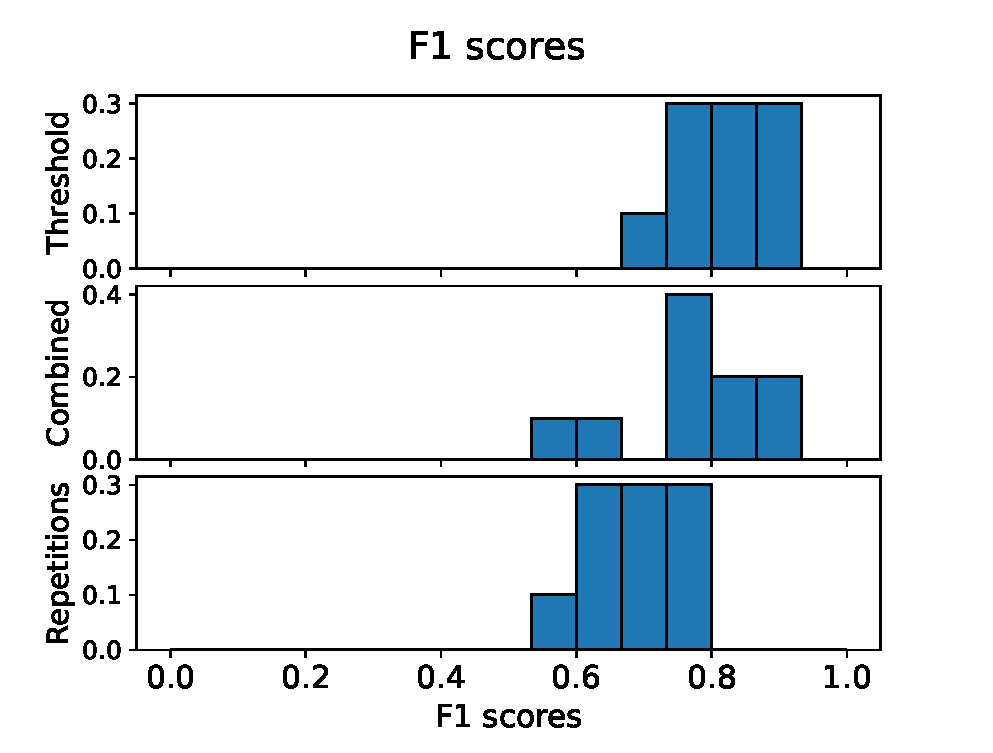
\includegraphics[width=\textwidth]{files/figs/res/femval/f1.eps}
    \caption{}
    \label{fig:femval-f1}
  \end{subfigure}

  \begin{subfigure}[t]{0.4\textwidth}
    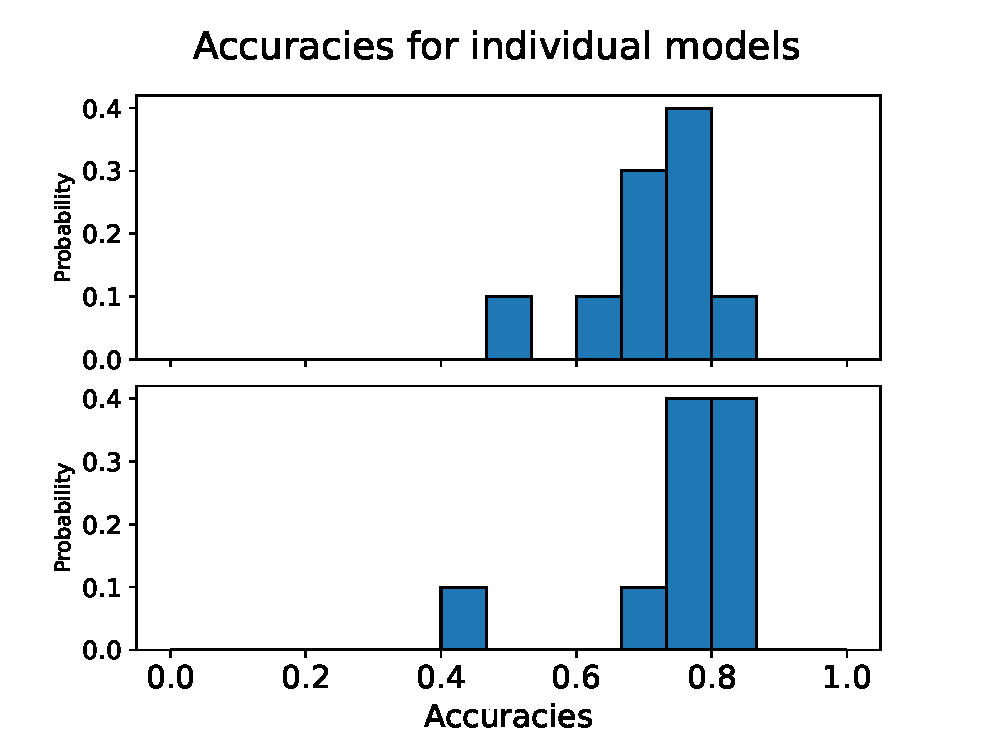
\includegraphics[width=\textwidth]{files/figs/res/femval/acc-ind.eps}
    \caption{}
    \label{fig:femval-acc-ind}
  \end{subfigure}
  ~
  \begin{subfigure}[t]{0.4\textwidth}
    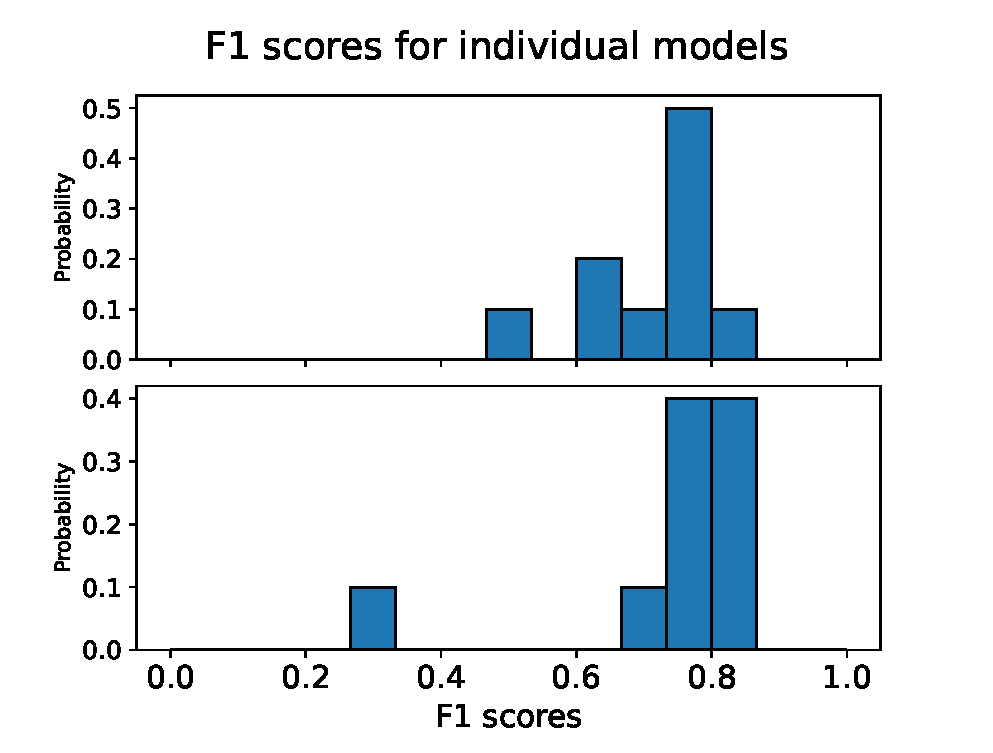
\includegraphics[width=\textwidth]{files/figs/res/femval/f1-ind.eps}
    \caption{}
    \label{fig:femval-f1-ind}
  \end{subfigure}
  \caption{Histograms of the accuracies and F1 scores summarized in Table \ref{tab:femval-results} along with the same metrics for the repetition classification for the models making up the ensembles, presented in Table \ref{tab:ensemble-models}. The high precision models only predicting one class are excluded.}
  \label{fig:femval-hist-results}
\end{figure}

% LAGG TILL FIGURE MED GRAD CAM!!!!!!

\begin{figure}
  \centering
  \begin{subfigure}[t]{0.33\textwidth}
    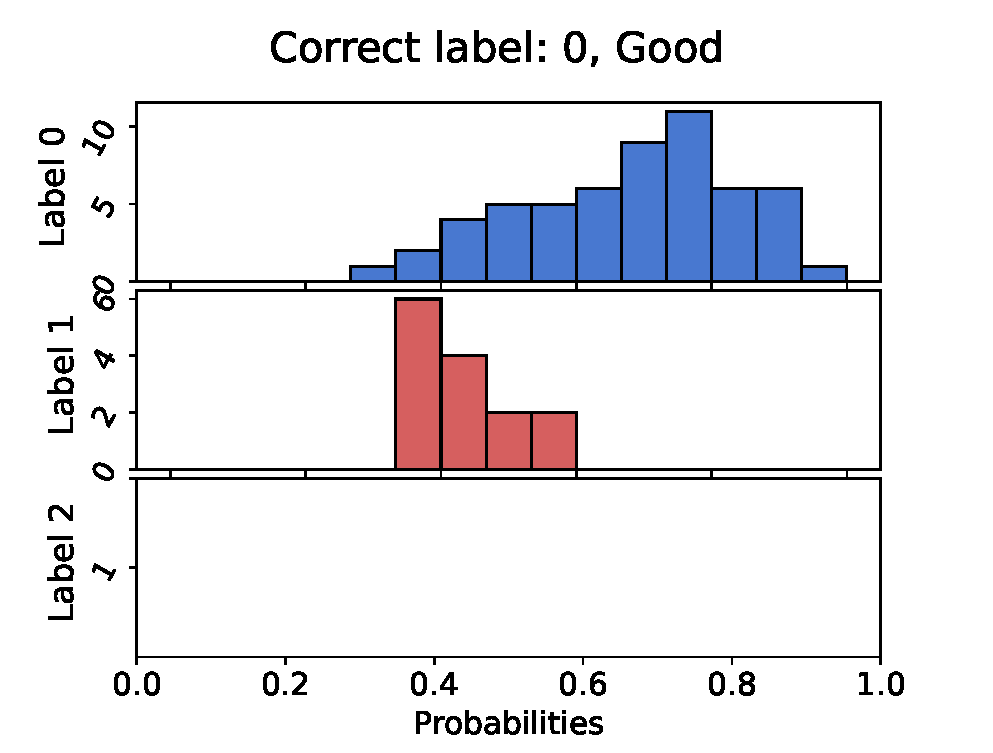
\includegraphics[width=\textwidth]{files/figs/res/femval/pc0-rb.eps}
    \caption{}
    \label{fig:femval-pc0}
  \end{subfigure}%
  \begin{subfigure}[t]{0.33\textwidth}
    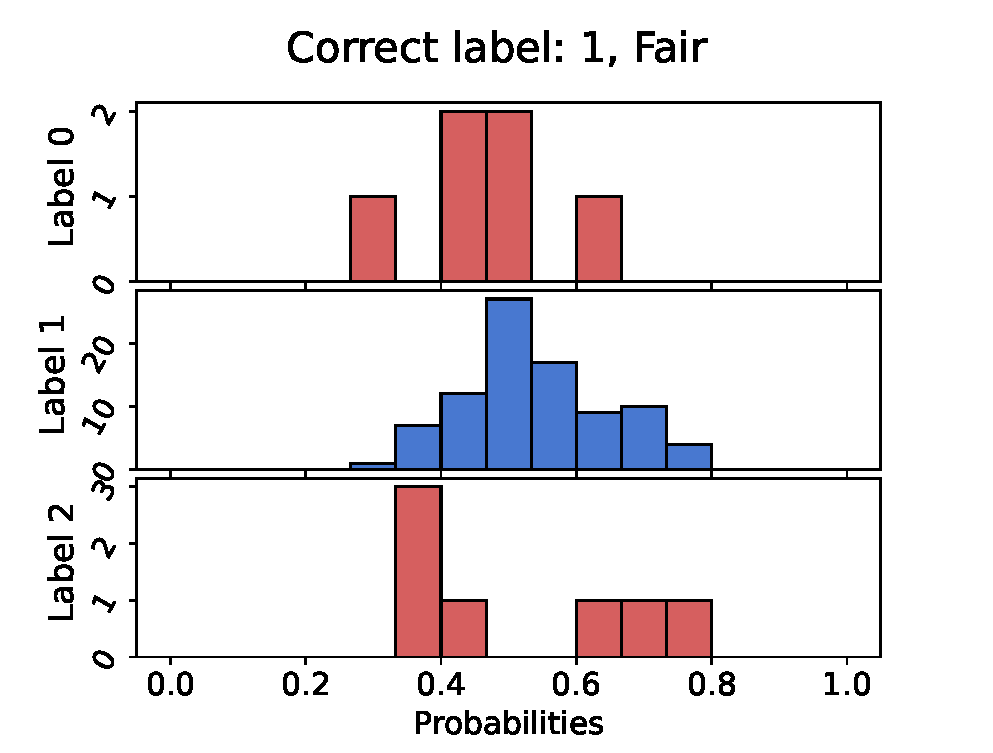
\includegraphics[width=\textwidth]{files/figs/res/femval/pc1-rb.eps}
    \caption{}
    \label{fig:femval-pc1}
  \end{subfigure}%
  \begin{subfigure}[t]{0.33\textwidth}
    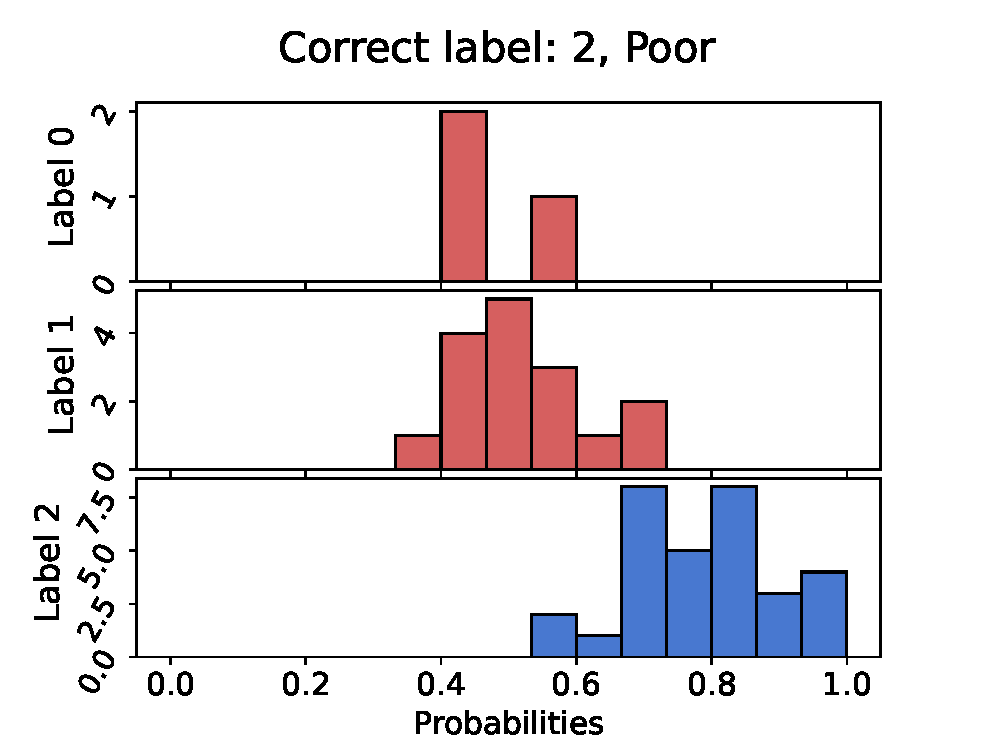
\includegraphics[width=\textwidth]{files/figs/res/femval/pc2-rb.eps}
    \caption{}
    \label{fig:femval-pc2}
  \end{subfigure}

  \caption{Figures showing the probabilities for the predicted class, i.e., the argmax of the model output, without threshold, for correct class 0: (a), 1: (b), and 2: (c). Incorrect predictions are shown in red.}
  \label{fig:femval-pc}
\end{figure}

As for the trunk model, the probability for class one is low. This is clearly not a problem for the classification, as mentioned above this model seems to be slightly biased towards class 1. It is however something to consider for the confidence score desirable in a clinical setting.


With the ensemble consisting of different models, some of the explainability from the X-InceptionTime architecture is lost. It is still possible to get importance values for each time step, but the regular models will not differentiate between the inputs. Figure~\ref{fig:gradcam} shows the activation maps for some different inputs to a single X-InceptionTime model, both for correctly and incorrectly classified samples. It can be seen how the same regions seems to be deemed important for the same predictions.%, but the importance is slightly higher when the prediction is correct.

\begin{figure}[h]
  \begin{subfigure}[t]{0.32\textwidth}
    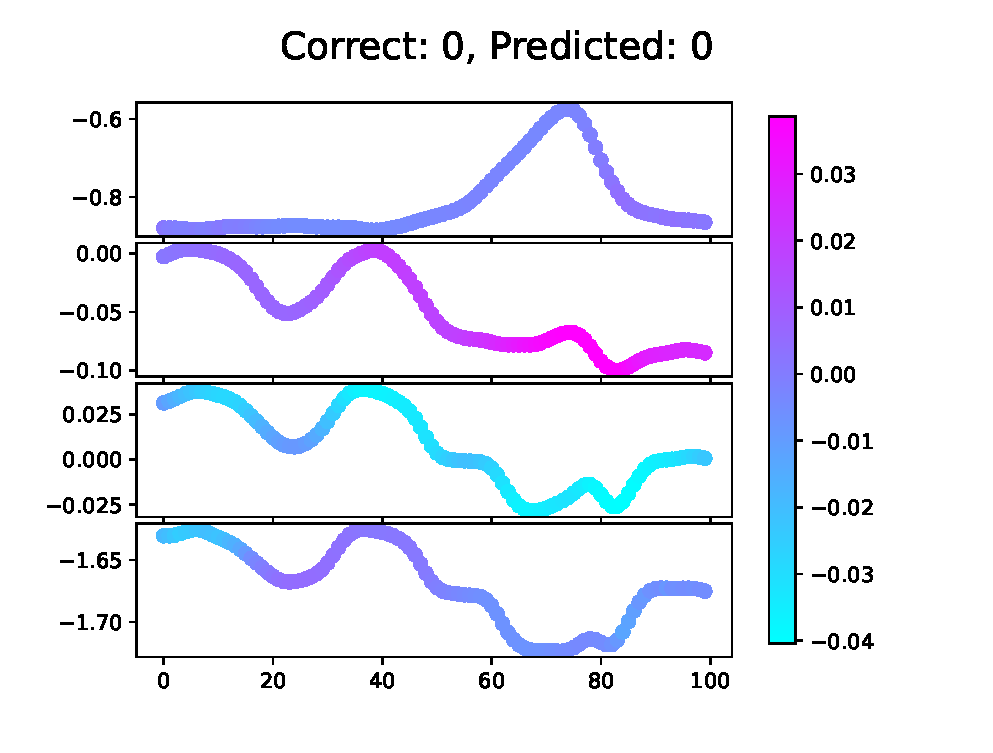
\includegraphics[width=\textwidth]{files/figs/res/femval/gradcam/00.eps}
    \caption{}
    \label{fig:femval-00}
  \end{subfigure}
  ~
  \begin{subfigure}[t]{0.32\textwidth}
    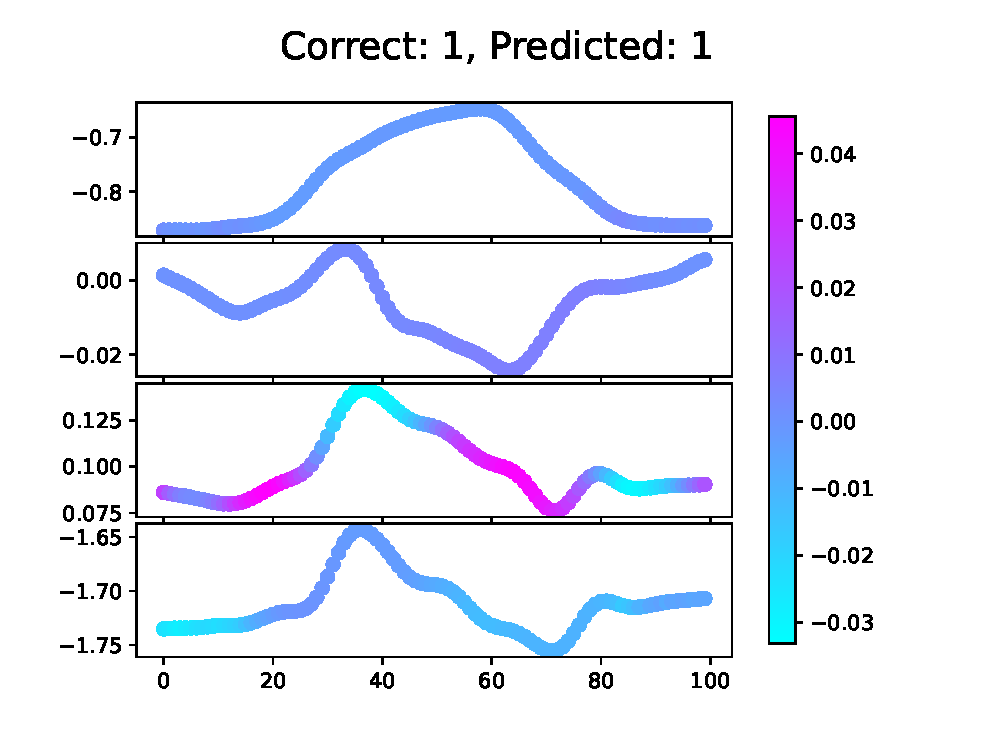
\includegraphics[width=\textwidth]{files/figs/res/femval/gradcam/11.eps}
    \caption{}
    \label{fig:femval-11}
  \end{subfigure}
  ~
  \begin{subfigure}[t]{0.32\textwidth}
    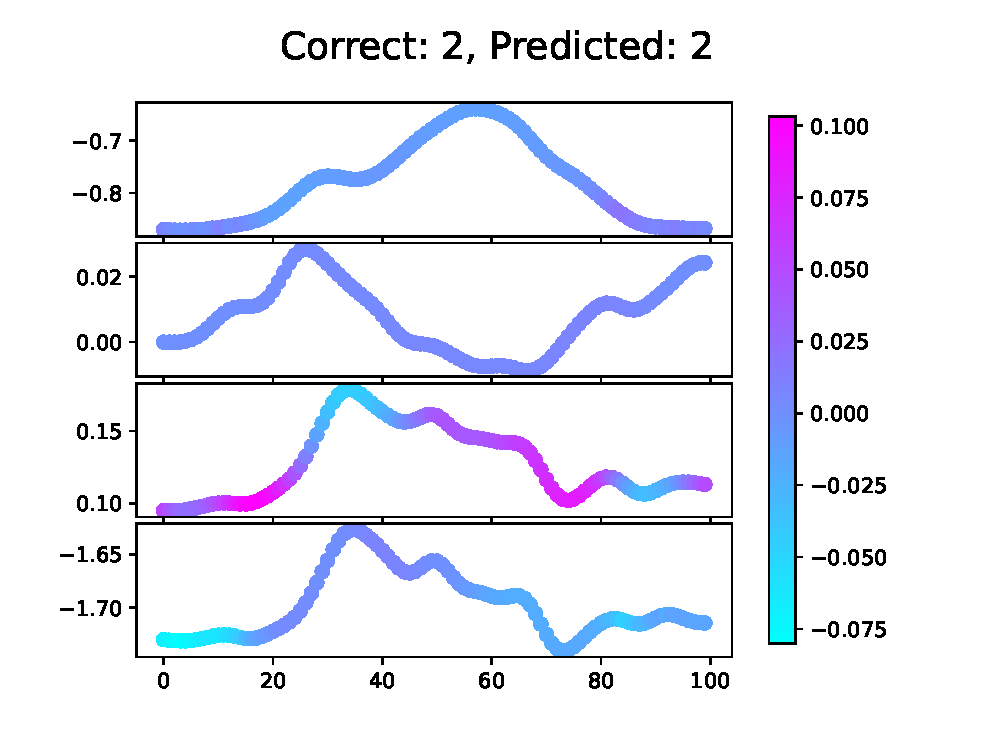
\includegraphics[width=\textwidth]{files/figs/res/femval/gradcam/22.eps}
    \caption{}
    \label{fig:femval-22}
  \end{subfigure}

  \begin{subfigure}[t]{0.32\textwidth}
    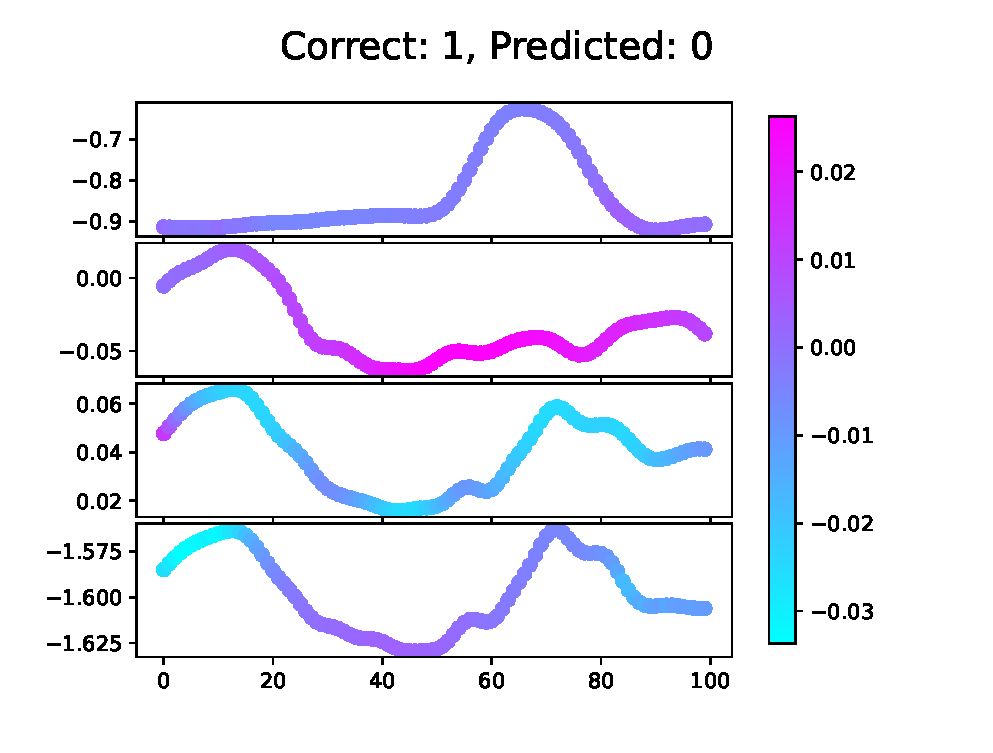
\includegraphics[width=\textwidth]{files/figs/res/femval/gradcam/10.eps}
    \caption{}
    \label{fig:femval-10}
  \end{subfigure}
  ~
  \begin{subfigure}[t]{0.32\textwidth}
    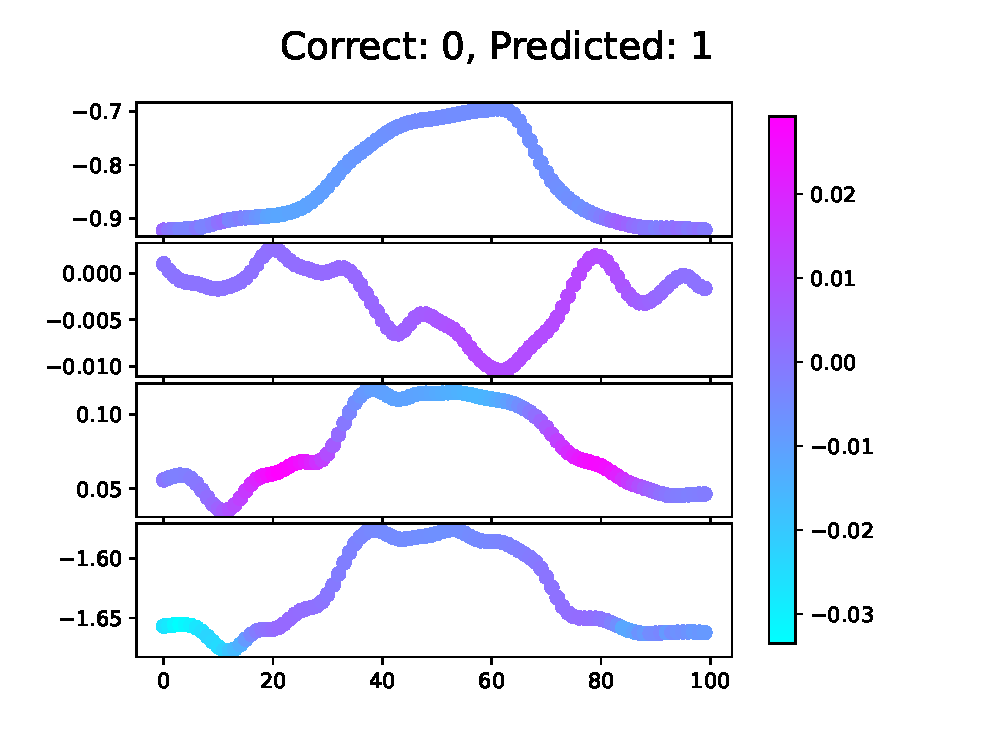
\includegraphics[width=\textwidth]{files/figs/res/femval/gradcam/01.eps}
    \caption{}
    \label{fig:femval-01}
  \end{subfigure}
  ~
  \begin{subfigure}[t]{0.32\textwidth}
    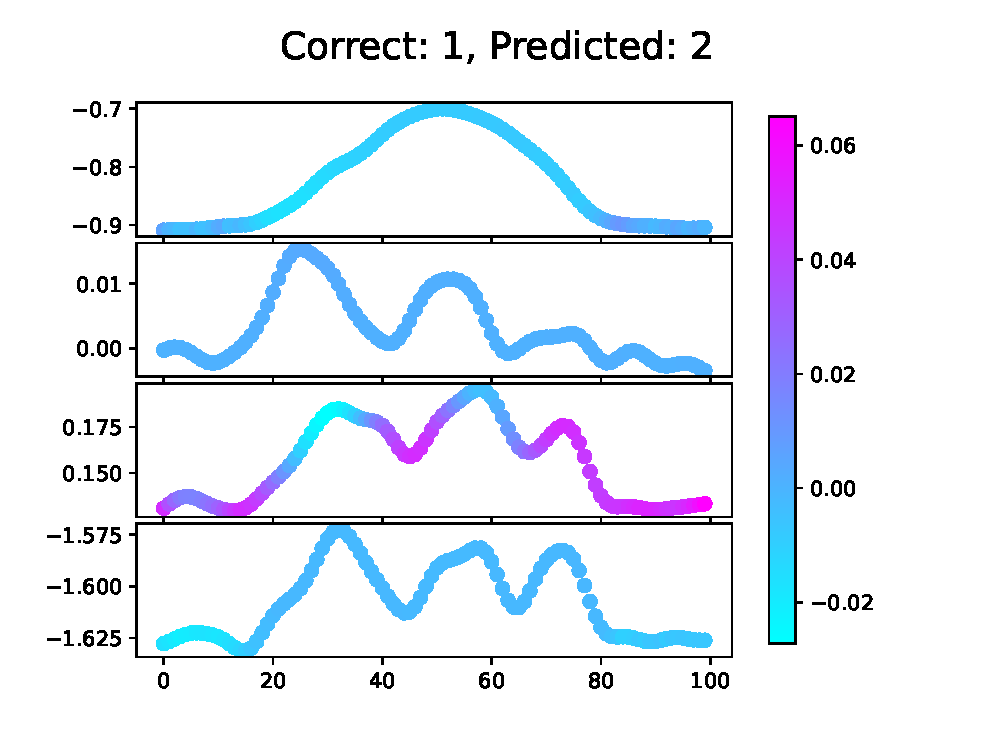
\includegraphics[width=\textwidth]{files/figs/res/femval/gradcam/12.eps}
    \caption{}
    \label{fig:femval-12}
  \end{subfigure}
  \caption{Activation maps applied to different inputs showing what was important for decision. The subplots show from the top: $y$ coordinate of the right shoulder, $x$ coordinate of the right hip, $x$ coordinate of the right knee, and angle between right knee and right ankle.}
  \label{fig:gradcam}
\end{figure}




\FloatBarrier
\subsection{Knee Medial-to-Foot Position}
As can be seen in Table~\ref{tab:kmfp-class-dist}, the \gls{kmfp} data is heavily unbalanced making it somewhat difficult to analyze. As long as this training set is a representable class distribution this model might perform satisfactory. However, it has seen very few examples of both class 1 and 2, so the risk of out-of-distribution samples if deploying this model is probably rather high. Regarding the performance metrics this model achieves a good accuracy which is natural since it will do so by just classifying most data as class 0. Based on the other metrics and the confusion matrices it becomes clear that it does not simply do this. To avoid such behavior some of the models used in the ensemble were slightly biased towards class 1 and 2. This shows in the result mainly as a low precision for class 1 compared to the other \glspl{poe}. The low standard deviation for the accuracy shows that the number of misclassification is similar for all examples. Due to the macro averaging of the other metrics together with the class imbalance, variations in a single classification of class 1 or 2 results in the large standard deviations seen for F1, recall, and precision.

%The threshold results in an average of 0.7 ignored sequences for this \gls{poe}.
% can be seen that it performs somewhat in line with
% The high variance in the F1 score is explained by the imbalanced data as any misclassification of class 1 or 2 will have a big effect on this. For this \gls{poe} an average of 0.7 sequences are ignored due to the threshold and 0.5 of these was correctly classified.

\begin{figure}[h]
  \centering
  \begin{subfigure}[t]{0.48\textwidth}
      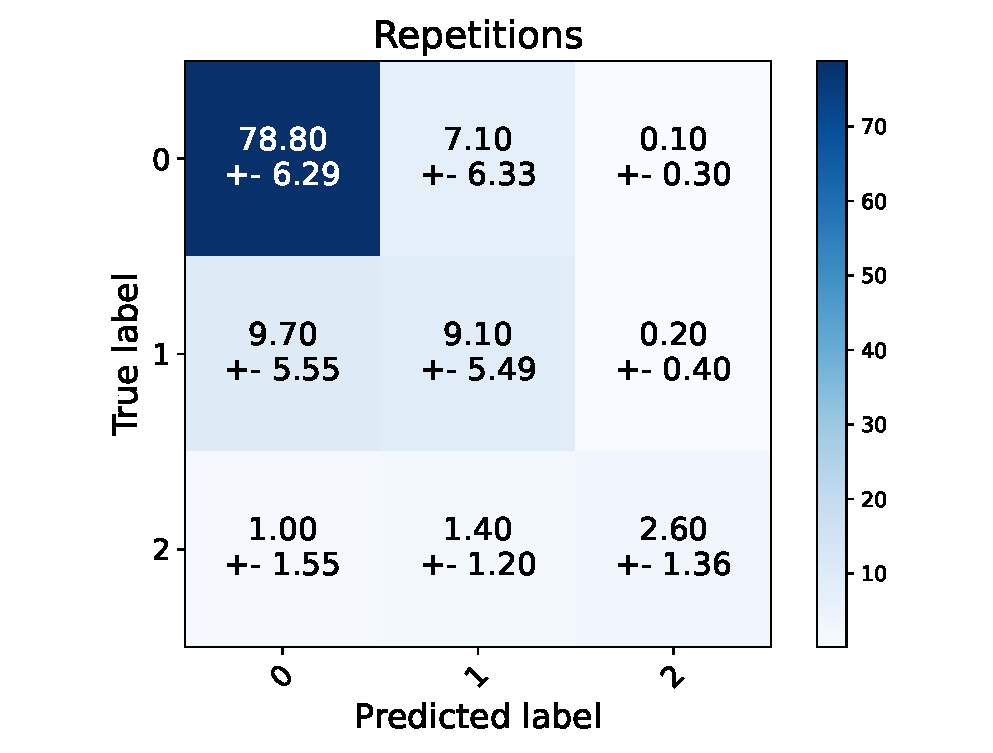
\includegraphics[width=\textwidth]{files/figs/res/kmfp/cnf-reps.eps}
      \caption{}
      \label{fig:kmfp-cnf-reps}
  \end{subfigure}
  ~
  \begin{subfigure}[t]{0.48\textwidth}
      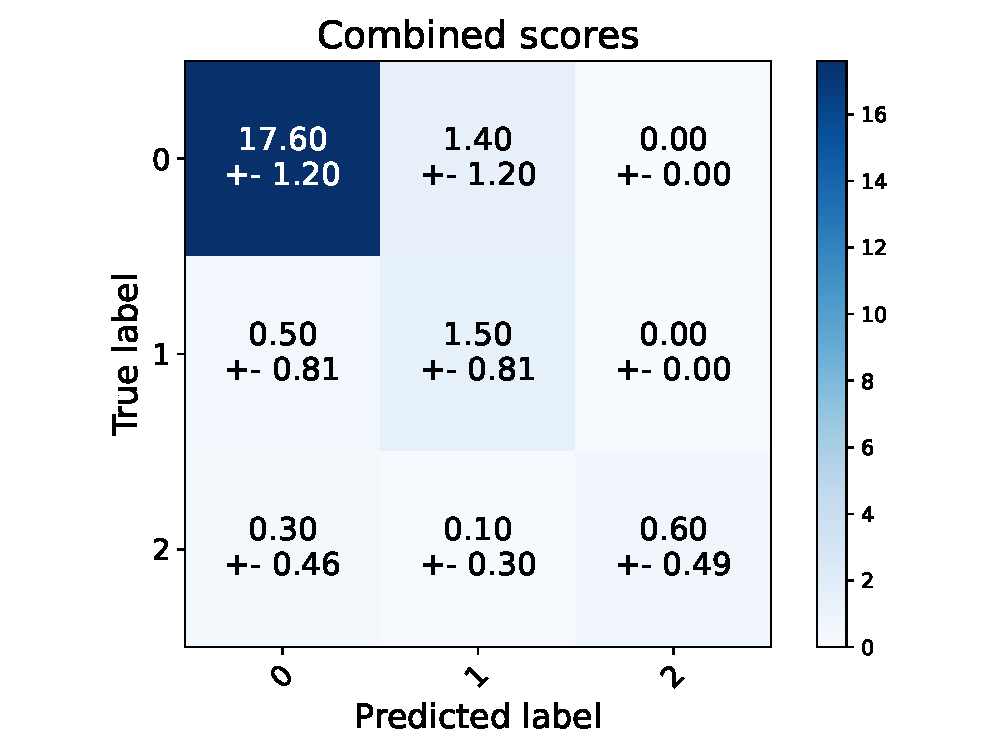
\includegraphics[width=\textwidth]{files/figs/res/kmfp/cnf-combined.eps}
      \caption{}
      \label{fig:kmfp-cnf-comb}
  \end{subfigure}

  \begin{subfigure}[t]{0.48\textwidth}
      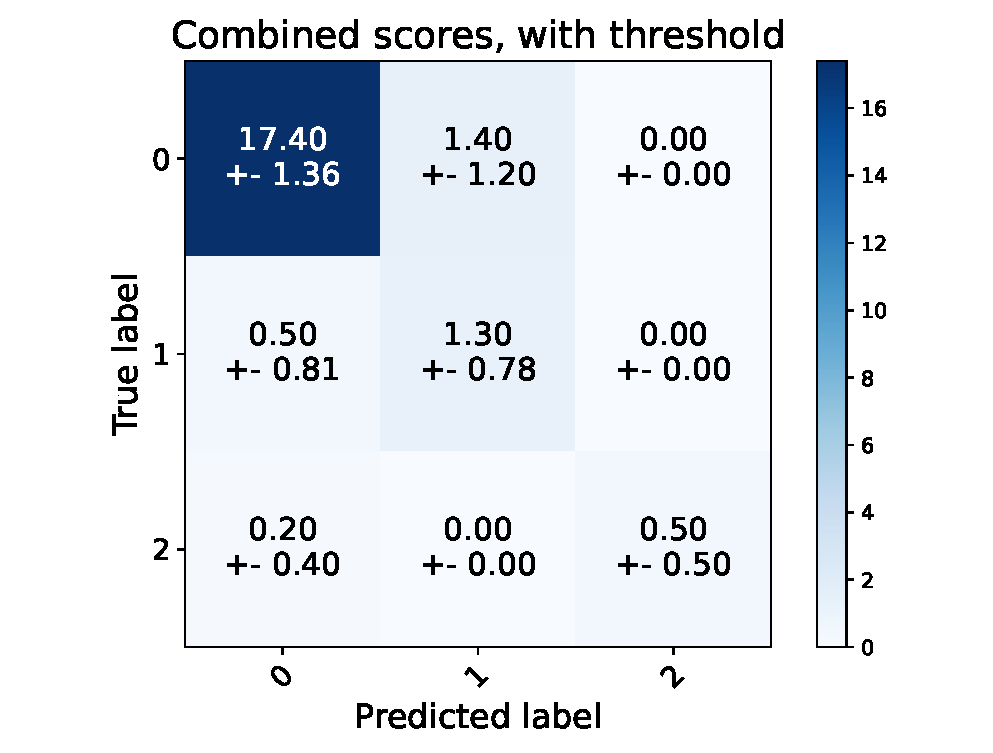
\includegraphics[width=\textwidth]{files/figs/res/kmfp/cnf-combined-th.eps}
      \caption{}
      \label{fig:kmfp-cnf-comb-th}
  \end{subfigure}
  ~
  \begin{subfigure}[t]{0.48\textwidth}
      \includegraphics[width=\textwidth]{files/figs/res/kmfp/cnf-ignored.eps}
      \caption{}
      \label{fig:kmfp-cnf-ignored}
  \end{subfigure}
  \caption{Confusion matrices for the KMFP classification on the test set. Classification of the individual repetitions is shown in (a), the combined score for the sequences of 5 repetitions is shown in (b). (c) shows the combined score with the threshold suggested in Section \ref{sec:met-combined}, i.e. all scores with a predicted probability higher than 0.4. The scores ignored due to this threshold are shown in (d). The entries in the matrices show the mean and standard deviation of the 10 ensembles trained in the cross validation.}
  \label{fig:kmfp-cnfs}
\end{figure}

\begin{table}[h]
  \caption{The class distribution in the test data for the KMFP POE.}
  \label{tab:kmfp-class-dist}
  \centering
  \begin{tabu}[c]{cccc}
    % \hline
    \textbf{Class}      & 0, Good & 1, Fair & 2, Poor \\ \hline \hline
    \textbf{Proportion (\%)} & 78.2 & 17.3 & 4.5 \\ %\hline
  \end{tabu}
\end{table}

\begin{table}
  \centering
  \caption{Results of the ensemble for the KMFP POE. Rep., Comb., and Thresh. represents the results for the repetitions, combinations, and combinations with thresholds, respectively. The Certainties columns show the results making up the Comb. column, but for the certainty levels of the expert labeling the data. These ranges from certain (0) to uncertain (2), the variable $n$ shows how many datapoints each category contains. All results are the mean from the 10 folds $\pm$ the corresponding standard deviations. F1, recall, and precision are macro averaged.}
  \label{tab:kmfp-results}
  \small
    \begin{tabu}[c]{|c|c|c|c||c|c|c|}
      \hline
      & \multirow{2}{*}{\textbf{Rep.}} & \multirow{2}{*}{\textbf{Comb.}} & \multirow{2}{*}{\textbf{Thresh.}} & \multicolumn{3}{c|}{\textbf{Certainties}}\\ \cline{5-7}
      & & & &0($n$=19)&1($n$=2)&2($n$=1)\\ \hline
      Accuracy (\%)   &82.3$\pm$3.1&89.5$\pm$4.5&\textbf{90.3$\pm$4.3}
                      &\textbf{92.6$\pm$5.3}&90.0$\pm$20.0&30.0$\pm$45.8\\ \hline
      F1 score (\%)   &65.1$\pm$13.7&69.0$\pm$24.6&\textbf{74.0$\pm$22.3}
                      &\textbf{69.3$\pm$28.6}&57.8$\pm$17.8&10.0$\pm$15.3\\ \hline
      Recall (\%)     &63.8$\pm$14.4&75.9$\pm$26.7&\textbf{81.1$\pm$24.7}
                      &\textbf{75.3$\pm$29.4}&60.0$\pm$13.3&10.0$\pm$15.3\\ \hline
      Precision (\%)  &\textbf{78.5$\pm$8.2}&66.1$\pm$24.0&71.4$\pm$22.6
                      &\textbf{67.2$\pm$28.9}&56.7$\pm$20.0&10.0$\pm$15.2\\ \hline
    \end{tabu}
\end{table}


\begin{figure}
  \centering
  \begin{subfigure}[t]{0.4\textwidth}
    \includegraphics[width=\textwidth]{files/figs/res/kmfp/acc.eps}
    \caption{}
    \label{fig:kmfp-acc}
  \end{subfigure}
  ~
  \begin{subfigure}[t]{0.4\textwidth}
    \includegraphics[width=\textwidth]{files/figs/res/kmfp/f1.eps}
    \caption{}
    \label{fig:kmfp-f1}
  \end{subfigure}

  \begin{subfigure}[t]{0.4\textwidth}
    \includegraphics[width=\textwidth]{files/figs/res/kmfp/acc-ind.eps}
    \caption{}
    \label{fig:kmfp-acc-ind}
  \end{subfigure}
  ~
  \begin{subfigure}[t]{0.4\textwidth}
    \includegraphics[width=\textwidth]{files/figs/res/kmfp/f1-ind.eps}
    \caption{}
    \label{fig:kmfp-f1-ind}
  \end{subfigure}
  \caption{Histograms of the accuracies and F1 scores summarized in Table \ref{tab:kmfp-results} along with the same metrics for the repetition classification for the models making up the ensembles, presented in Table \ref{tab:ensemble-models}. The high precision models only predicting one class are excluded.}
  \label{fig:kmfp-hist-results}
\end{figure}


\begin{table}
  \caption{With what confidence different measures led to improvements, i.e, a higher number means we can be more certain that the performance is increased by performing the corresponding measure. Calculated assuming normal distributions and using pairwise comparisons for the folds. When comparing the ensemble with the individual models the best model is chosen.}
  \label{tab:kmfp-improvements}
  \centering
  \begin{tabu}[c]{|c|c|c|c|}
    \hline
    & \multicolumn{1}{c|}{\begin{tabular}[c]{@{}c@{}}\textbf{Ensemble -}\\\textbf{individual} \\\textbf{models}\end{tabular}} &
    \multicolumn{1}{c|}{\begin{tabular}[c]{@{}c@{}}\textbf{Combined -}\\\textbf{Repetitions}\end{tabular}} &
    \multicolumn{1}{c|}{\begin{tabular}[c]{@{}c@{}}\textbf{Threshold -}\\\textbf{Combined}\end{tabular}} \\ \hline
    \textbf{Accuracy} & - & 95\% & 95\% \\ \hline
    \textbf{F1 score} & - & 95\% & 95\% \\ \hline
  \end{tabu}
\end{table}


\begin{figure}
  \centering
  \begin{subfigure}[t]{0.33\textwidth}
    \includegraphics[width=\textwidth]{files/figs/res/kmfp/pc0-rb.eps}
    \caption{}
    \label{fig:kmfp-pc0}
  \end{subfigure}%
  \begin{subfigure}[t]{0.33\textwidth}
    \includegraphics[width=\textwidth]{files/figs/res/kmfp/pc1-rb.eps}
    \caption{}
    \label{fig:kmfp-pc1}
  \end{subfigure}%
  \begin{subfigure}[t]{0.33\textwidth}
    \includegraphics[width=\textwidth]{files/figs/res/kmfp/pc2-rb.eps}
    \caption{}
    \label{fig:kmfp-pc2}
  \end{subfigure}

  \caption{Figures showing the probabilities for the predicted class, i.e., the argmax of the model output, without threshold, for correct class 0: (a), 1: (b), and 2: (c). Incorrect predictions are shown in red.}
  \label{fig:kmfp-pc}
\end{figure}

\FloatBarrier
\subsection{Summary}
The results with their 95\% confidence intervals are summarized in Table \ref{tab:sum-ci}. These confidence intervals assumes Gaussian distributions, which is not unrealistic for trunk, femoral valgus, and to some extent \gls{kmfp}. For the pelvis however, this assumption does not seem to be very reasonable. Based on this, it can be said that the model for femoral valgus seems to perform the best followed by trunk. \gls{kmfp} achieves a high accuracy, but it is difficult to draw any conclusions about the performance for the Fair (1) or Poor (2) classes due to the very few examples. The pelvis model does not perform very well which might be due to that it is based on information not available in the 2D joint position data. For all \glspl{poe} the developed models clearly outperforms the baseline methods.

The only difference between the different fold models is a slight variation in the training data. Still, the result, generated on the same testing data, clearly varies. This suggests that more data would be very welcome for all models. Both to improve the performance through bigger training sets and to give more reliable evaluations thanks to more testing data.

\begin{table}[h]
  \caption{Approximative 95\% confidence intervals for the performance of the combined scores with thresholds for different POEs, assuming Gaussian distributions. }
  \label{tab:sum-ci}
  \centering
  \begin{tabu}[c]{|c|c|c|c|c|}
    \hline
    & \textbf{Trunk} & \textbf{Pelvis} &\textbf{Femoral Valgus} & \textbf{\gls{kmfp}} \\ \hline
    \textbf{Accuracy (\%)}  & 80.0$\pm$4.9 & 73.3$\pm$11.9 & 82.3$\pm$3.8 & \textbf{90.3$\pm$2.7} \\\hline
    \textbf{F1 score (\%)}  & 79.9$\pm$5.6 & 73.6$\pm$14.1 & \textbf{81.0$\pm$3.3} & 74.0$\pm$14.1 \\ \hline
    \textbf{Recall (\%)}    & \textbf{81.6$\pm$4.6} & 77.9$\pm$9.4  & 79.5$\pm$3.5 & 81.1$\pm$15.6 \\ \hline
    \textbf{Precision (\%)} & 83.0$\pm$4.3 & 74.9$\pm$15.1 & \textbf{86.5$\pm$3.5} & 71.4$\pm$14.3 \\\hline
  \end{tabu}
\end{table}

Regarding the model selection, it is notable that padded and normalized data yields similar results. This suggests that, at least with this amount of data, the frequency content or the speed of the movements is not an indicator of the \gls{poe} score. Instead, the overall shape of the movements of the different body parts are important, which matches the descriptions in Appendix~\ref{app:poe-task}. Normalizing the data length probably unifies these shapes slightly over all data, which might make it easier to find patterns.

Another thing to note is that deep models does not seem to be effective as models with depths of one and two performed the best. Similarly, the InceptionTime model where interactions between the inputs are taken into account does not perform significantly better than X-InceptionTime. This suggests, at least with this amount of data, that the discriminating features are not that complicated and does not depend on direct interactions between the inputs, apart from difference or angles in some cases. With more data this might be different as new patterns could be found.
